\documentclass[10pt,twocolumn]{article}

\usepackage[T1]{fontenc}
\usepackage{lmodern}
\usepackage{microtype}
\usepackage[margin=0.68in,columnsep=0.27in]{geometry}
\usepackage{amsmath,amssymb,amsthm,mathtools}
\usepackage{booktabs}
\usepackage{tabularx}
\usepackage{array}
\usepackage{enumitem}
\usepackage{xcolor}
\usepackage{tikz}
\usepackage{listings}
\usepackage{hyperref}
\usetikzlibrary{arrows.meta,positioning,calc,fit}

\definecolor{Ink}{HTML}{17252C}
\definecolor{Slate}{HTML}{475A63}
\definecolor{Muted}{HTML}{738188}
\definecolor{Rule}{HTML}{D7DEDF}
\definecolor{Panel}{HTML}{F3F6F6}
\definecolor{Accent}{HTML}{0B7781}
\definecolor{AccentSoft}{HTML}{E6F2F2}
\definecolor{Fault}{HTML}{A7433B}
\definecolor{FaultSoft}{HTML}{F8ECEA}
\definecolor{Amber}{HTML}{A66A12}
\definecolor{AmberSoft}{HTML}{F8F0E3}

\hypersetup{
  colorlinks=true,
  linkcolor=Accent,
  urlcolor=Accent,
  citecolor=Accent,
  pdftitle={UNO: Coordinator-Free Crash-Atomic Publication over Ordinary Blobs},
  pdfauthor={Commonware storage design note}
}

\setlength{\parindent}{1em}
\setlength{\parskip}{0pt}
\setlist{nosep,leftmargin=*}
\setlist[description]{style=nextline,font=\normalfont\bfseries}
\renewcommand{\arraystretch}{1.08}

\newtheorem{definition}{Definition}
\newtheorem{assumption}{Assumption}
\newtheorem{invariant}{Invariant}
\newtheorem{lemma}{Lemma}
\newtheorem{theorem}{Theorem}
\newtheorem{conjecture}{Conjecture}
\newtheorem{corollary}{Corollary}
\newtheorem{proposition}{Proposition}
\theoremstyle{remark}
\newtheorem{remark}{Remark}
\newtheorem{limitation}{Limitation}

\newcommand{\code}[1]{\texttt{#1}}
\newcommand{\old}{\mathsf{old}}
\newcommand{\new}{\mathsf{new}}
\newcommand{\absent}{\bot}
\newcommand{\Root}{\mathsf{R}}
\newcommand{\Prepared}{\mathsf{B}}
\newcommand{\Materialized}{\mathsf{M}}
\newcommand{\Tombstone}{\mathsf{T}}
\newcommand{\Abort}{\mathsf{A}}
\newcommand{\Zero}{\mathsf{Z}}
\newcommand{\Valid}{\mathsf{Valid}}
\newcommand{\Durable}{\mathsf{Durable}}
\newcommand{\Complete}{\mathsf{Complete}}
\newcommand{\Final}{\mathsf{Final}}
\newcommand{\keyof}{\mathsf{key}}
\newcommand{\inc}{\iota}
\newcommand{\gid}{\gamma}
\newcommand{\crc}{\mathsf{CRC32C}}
\newcommand{\bytes}{\mathsf{bytes}}
\newcommand{\view}{\mathsf{view}}
\newcommand{\sync}{\mathsf{sync}}
\newcommand{\dirsync}{\mathsf{dirsync}}
\newcommand{\unlink}{\mathsf{unlink}}
\newcommand{\kw}[1]{\textbf{#1}}

\lstdefinestyle{protocol}{
  basicstyle=\ttfamily\footnotesize,
  keywordstyle=\bfseries\color{Accent},
  commentstyle=\itshape\color{Muted},
  frame=single,
  rulecolor=\color{Rule},
  backgroundcolor=\color{Panel},
  columns=fullflexible,
  keepspaces=true,
  showstringspaces=false,
  breaklines=true,
  xleftmargin=0.2em,
  xrightmargin=0.2em,
  aboveskip=0.6em,
  belowskip=0.6em
}

\tikzset{
  box/.style={draw=Rule,fill=white,line width=.55pt,minimum height=.62cm,align=center,inner xsep=.12cm,inner ysep=.08cm},
  root/.style={draw=Accent,fill=AccentSoft,line width=.7pt,minimum height=.62cm,align=center,inner xsep=.12cm,inner ysep=.08cm},
  warn/.style={draw=Amber,fill=AmberSoft,line width=.65pt,align=center,inner sep=.12cm},
  bad/.style={draw=Fault,fill=FaultSoft,line width=.65pt,align=center,inner sep=.12cm},
  flow/.style={-{Latex[length=2mm,width=1.2mm]},draw=Accent,line width=.75pt},
  faint/.style={draw=Muted,line width=.55pt}
}

\title{\vspace{-1.2em}\textbf{UNO: Coordinator-Free Crash-Atomic Publication\\over Ordinary Blobs}}
\author{Commonware storage design note}
\date{7 August 2026}

\begin{document}
\maketitle

\begin{abstract}
UNO is an append-oriented storage design for atomically publishing pending epochs of several
ordinary blobs without a coordinator file, root WAL, or shared allocation layer. Payload is written
once at its final offset. Each participant stores one checksummed local witness beside an otherwise
invisible prepared root; witnesses form a canonical successor ring. The normative R14-2P reference
protocol treats a complete, valid ring as the commit decision and publishes it in two ordered
durability layers per participant: first all non-guard slot bytes and the candidate payload/length
evidence, then only the one-byte generation-colored prepared guard. Each layer may fan out across
files; no coordinator record or cross-file barrier is introduced.

This paper specifies a target transition system using generation-colored root spellings under a crash model
in which \emph{any subset} of non-durable addressed writes may survive---not merely a prefix of
submission order. It states the assumptions and invariants, gives a separate argument for rings
broken after deletion finalization, derives bounded-recovery and acknowledged-durability targets,
and identifies the cases outside the intended theorem. In particular,
absence is never a prepare vote. No path may disappear until every participant has an independent,
durable final root. Thereafter each retained root selects the new value and each tombstone
independently denotes logical absence, so out-of-order cleanup can strand physical garbage but
cannot expose a mixed vector. The checked-in implementation is compared against that target rather
than assumed to satisfy it. The audit exposes concrete refinement blockers, including stale-ring
authority and unconsumed rejected witnesses, and records the reviewed repair for a filesystem-
backend cancellation defect; \S\ref{sec:implementation-status} states the distinction explicitly.
The former one-phase R14-1P proposal and checked-in generation-uncolored R13 format remain explicit
nonconforming controls. R14-1P can splice an older witness topology with newly issued candidate
bytes into an exact, never-issued smaller ring. R14-2P closes that provenance gap by ordering the
only write of the $B$ guard after the exact body and payload evidence are durable, clearing all live
phase credit on crash, and forbidding recovery from writing $B$. The result is a reviewable
reference specification and a manual safety conjecture. The current 42-harness Kani matrix is
pending for its exact source snapshot; completed 30- and 36-harness matrices apply only to older
snapshots. The physical, composed, and protocol abstractions remain separate, and an end-to-end
refinement theorem and production refinement remain absent.
\end{abstract}

\noindent\fcolorbox{Accent}{AccentSoft}{%
  \parbox{\dimexpr\columnwidth-2\fboxsep-2\fboxrule\relax}{\small
  \textbf{Status.} UNO is an opt-in ALPHA API. Ordinary blob APIs and formats are unchanged.
  The append/rewind mechanism corresponds in part to the current code, while the root format and
  two-phase prepare below are the proposed R14-2P reference. Conjecture~\ref{thm:atomic} is stated
  for that transition system; its current bounded Kani obligations are pending, and the abstraction
  layers are not joined by one mechanized refinement theorem. R14-1P is retained only as a
  witness-splicing negative control, and R13 is a nonconforming implementation baseline.
  Current implementation deviations---including stale-ring
  authority, rejected-witness reuse, one integrity-boundary error, and unenforced
  direct-file/no-alias namespace preconditions---are listed in
  \S\ref{sec:implementation-status}. That section separately records a reviewed cancellation-
  ownership repair; no R14 conformance claim follows from that narrower fix.}}

\section{Problem and scope}

Journal-shaped structures commonly need one logical mutation to change several append-only byte
sequences: values and offsets, data and an index, or the active tails of several sections. If each
file publishes independently, a crash can expose a mixed vector. A conventional coordinator WAL
solves this by introducing another durable authority and at least one ordering edge. UNO instead
places a local fragment of the decision in every participant and makes the fragments mutually
discoverable.

The development name ``UNO'' denotes the target of writing payload \emph{once}, not a promise of
one durability layer. R14-2P has two serial per-participant durability layers. Within each layer an
$n$-participant group still has $n$ independent file obligations that may be submitted
concurrently. This is not a claim that one system call or one physical device flush occurs.

\subsection{Supported mutation vocabulary}

The current public batch vocabulary is:
\begin{itemize}
  \item \textbf{publish}: expose a participant's pending append/tag epoch;
  \item \textbf{rewind}: publish a non-increasing encoded length, never an extension; and
  \item \textbf{remove}: delete the current exact blob incarnation.
\end{itemize}
Blob creation and whole-partition deletion are not group operations. Arbitrary
positioned overwrite is also excluded: once a byte is committed, a later epoch may retain it or
exclude it by rewinding, but may not replace it in place. This restriction is what permits
write-once payload without undo data, page maps, hole management, or compaction.

\subsection{Events, observations, and safety target}

Let group $G$ target the ordered logical-key set
$K_G=\langle k_0,\ldots,k_{n-1}\rangle$ and the exact physical participants
$P_G=\langle p_0,\ldots,p_{n-1}\rangle$ occupying those keys when $G$ is validated. For each key,
$O_i$ is its caller-observable selected value---encoded length, integrity state, application tag,
and exact encoded payload bytes---before $G$, while $N_i$ is the corresponding candidate value
($\absent$ for a removal). Internal root generation, spelling, and witness bytes are deliberately
outside this logical projection.

For any mutating operation $H$, $\mathsf{admit}(H)$ is its first issued root, witness, or namespace
update that can affect crash recovery after validation and lock acquisition. Staging an append or
preflushing invisible payload is not admission because it cannot change a selected root. The
following group events are distinct:
\begin{description}
  \item[Admission $\mathsf{admit}(G)$.] For a group, the generic admission event is the first byte
  of a $G$-specific phase-1 slot body. A guardless phase-1 image is not a prepare vote, but remains
  an admission effect that recovery must resolve before mutation or reuse.
  \item[Decision $\mathsf{decide}(G)$.] Either every participant's phase-2 prepared-guard
  durability operation has succeeded, or crash recovery has read and validated a complete exact
  $B$-proven ring including every required payload byte. Once established, this is a monotone
  protocol fact.
  \item[Acknowledgement $\mathsf{ack}(G)$.] \code{start\_apply} returns \code{Ok}. This transition is
  permitted only after the normal phase-2 guard-barrier route has established
  $\mathsf{decide}(G)$.
  \item[Completion $\mathsf{complete}(G)$.] The returned handle resolves successfully after the
  in-memory state is active and required eager materialization, truncation, and namespace work has
  finished. Completion is not the durability linearization point.
\end{description}

A failed attempt to establish $\mathsf{decide}(G)$ is not the opposite monotone event. In
particular, a recognizable candidate generation or non-quiescent higher-generation image that does
not currently prove a candidate is only \emph{provisionally rejected} until an exact code-last $A$
root consumes that generation. Recovery re-decodes after a crash during the non-guard abort-body
write and honors any already-issued $B$ or final evidence that remains. It never supplies a missing
$B$ guard, so a guardless phase-1 body cannot be promoted into a decision. Recovery
returns the predecessor for caller mutation, truncates or overwrites payload, or reuses its slot only
after exact $A$; proof-preserving predecessor finalization remains permitted and may be required
before $A$. The sole no-$A$ case is a complete slot
that is byte-for-byte the canonical lower-generation pre-attempt source, including any exact witness
belonging to that lower generation, so no distinguishable candidate-generation admission effect
remains to consume. Once exact $A$ exists, the old outcome is irreversible for the consumed
generation.

For a crash image $D$, $\view_G(D)$ is the vector returned by a \emph{successful} fresh namespace
recovery followed by ordinary root recovery, before the caller optionally recreates an absent key.
A retained key maps to its selected metadata and payload bytes. An exact tombstone, or a missing
removed incarnation whose absence was produced by authorized post-finalization cleanup or a later
serialized remove, maps to $\absent$; internal generation/spelling is projected away. An actually
missing pre-finalization path is an assumption violation, not an old-vector encoding. A recovery
that detects corruption and fails closed returns
no vector and cannot be mistaken for either outcome. Under the stated assumptions, a crash image
created solely by protocol transitions has a defined recovery vector; fail-stop is reserved for an
assumption violation or a subsequent I/O failure. For one fixed disk image recovery is
deterministic; ``old or new'' below quantifies over the different disk images allowed by the crash
model.

\begin{definition}[Group crash atomicity]\label{def:atomic}
After $\mathsf{admit}(G)$ and before admission of any later create, publish, rewind, exact remove,
or whole-partition remove whose target contains a key in $K_G$, every protocol-reachable crash image
recovers to a vector satisfying
\[
  \view_G(D) \in \{\langle O_0,\ldots,O_{n-1}\rangle,
                      \langle N_0,\ldots,N_{n-1}\rangle\}.
\]
An admitted but unacknowledged group may yield either vector across allowed crash images. Every
image after $\mathsf{ack}(G)$ must yield the new vector.
\end{definition}

The definition is crash/reopen atomicity, not live read isolation. Existing handles may expose
pending bytes according to the API, and recreation is a later key mutation rather than part of the
recovered absence observation. After a later conflicting operation is admitted, the old/new-only
interval ends. The stronger remaining obligation is that recovery correspond to a serial history in
which a decided $G$ appears completely before that operation, while a rejected $G$ contributes no
state transition and the later operation follows its predecessor state. UNO intentionally defines
no total durable order between disjoint groups. A semantic dependency must be placed in one group or
ordered by waiting for the first acknowledgement.

\section{System and fault model}

\subsection{Objects and identities}

A storage namespace is exclusively owned by one storage instance and its clones. A logical key is
$k=(q,x)$, where $q$ is a UTF-8 partition string and $x$ is an uninterpreted blob-name byte string.
Keys are ordered lexicographically by $q$ and then by raw bytes of $x$.

A physical participant is
\[
  p=(k,\inc,f),
\]
where $\inc\in\{0,1\}^{128}$ is the immutable incarnation in the file header and $f$ is the current
directly named regular-file inode at $k$; following a symbolic link never yields a participant.
Recreating the same key mints a new incarnation. Protocol records always identify
both $k$ and $\inc$; unlink additionally checks the opened and current device/inode identity.
An ordinary non-atomic recreation may instead create a V1 blob with no UNO incarnation; it is a
fresh named inode generation and cannot be mistaken for the exact V2 participant.

\subsection{Medium operations}

The proof uses the following abstract interface.
\begin{description}
  \item[$\mathsf{write}(f,o,b)$] issues bytes $b$ at file offset $o$.
  \item[$\mathsf{truncate}(f,L)$] issues a file-length change to $L$ and preserves bytes below $L$.
  \item[$\sync(f)$] is a file durability barrier. On success, all earlier writes issued to $f$ are
  durable together with the last earlier issued file length and the metadata required to retrieve
  them.
  \item[$\unlink(k)$] removes a directory entry but may not yet make that absence crash-durable.
  \item[$\dirsync(q)$] makes earlier namespace changes in partition directory $q$ durable.
\end{description}
A durable positioned write such as Linux \code{pwritev2(RWF\_DSYNC)} is a scoped durability
operation: on success at least its addressed bytes and required retrieval metadata enter the durable
base. The implementation may persist unrelated dirty data too, but the proof takes no durability
credit for it. UNO uses that weaker obligation only where the candidate does not depend on those
unrelated bytes, such as a deletion candidate naming the prior committed payload.
A write beyond the current end also issues the length extension needed to address its bytes. When a
retained extension is reached in issue order, it first zero-initializes the offsets newly exposed at
that point; retained addressed-byte updates belonging to the extending write are then applied. Thus
if the extension survives without every byte of that write, the gap and the missing addressed cells
read as zero, matching Linux hole and unwritten-extension semantics; this zero-fill is part of the
length operation rather than invented medium damage. Bytes beyond the selected end remain
inaccessible and cannot satisfy candidate validation. A selected shrinking truncate preserves the
prefix and discards the old tail. Any later extension exposes zeros, and UNO assigns fresh write
stamps rather than treating discarded tail contents as durability credit.

\begin{assumption}[Arbitrary-subset addressed-write crash model]\label{a:fault}
For each file, a successful barrier establishes a durable base equal to applying every prior issued
byte update and length change in issue order. At a later crash, the recovered file is obtained by
starting from that base, retaining any subset of subsequently issued addressed-byte updates and
length changes, and applying the retained updates in issue order. Selection is independent by byte,
offset, and file; a multi-byte write may tear arbitrarily. Thus an overlapping byte is either its
last barrier-established value or a value subsequently issued to that address, never a value
superseded before the barrier. The medium does not invent values or damage an unaddressed byte.
Directory-entry durability is independent: before a directory barrier, any subset of subsequent
namespace updates may survive; after it, all earlier updates do. The recovered crash image becomes
the durable base for the next execution, so a byte observed after restart is not again treated as a
pre-crash volatile update.
\end{assumption}

This is strictly stronger than a prefix model: the second half of a root may survive while the
first does not, and participant $p_7$ may survive while $p_2$ does not. Every protocol write,
including recovery normalization, abort publication, final-root repair, truncation, and namespace
cleanup, is subject to the same rule. Recovery has no atomic-write privilege.

\begin{assumption}[Trusted local medium]\label{a:trusted}
The disk and namespace are not controlled by an adversary. CRC32C is modeled as collision-free for
the bytes encountered in an execution: a byte string different from every checksummed spelling
actually encoded by the protocol does not validate merely through a checksum collision. Exact
reconstruction is \emph{not} excluded. If a torn later write supplies common constant bytes while
older bytes supply the remainder of an earlier valid spelling, that spelling may validate and the
protocol must handle it. The implementation uses CRC32C to detect tears and accidental corruption,
not to authenticate data. Any safety claim is therefore probabilistic and conditional on this
validity event and on the medium honoring completed barriers. This assumption does not exclude the
exact old/new witness reconstruction in Limitation~\ref{l:witness-provenance}.
\end{assumption}

\subsection{Linux/ext4 refinement boundary}

The transition system is not an ext4 implementation model. It is an application-visible contract
that a backend must refine. On Linux, a successful \code{fdatasync} is used as the file barrier:
Linux includes file size and other metadata required to retrieve the data in that operation, while
an \code{fsync} of the file alone does not necessarily persist its directory entry. The latter
requires an explicit parent-directory \code{fsync}.\footnote{Linux \code{fsync(2)}:
\url{https://man7.org/linux/man-pages/man2/fsync.2.html}.} A range-scoped
\code{pwritev2(RWF\_DSYNC)} provides the per-write \code{O\_DSYNC} obligation for the addressed
range; it is not \code{RWF\_ATOMIC} and supplies no torn-write protection. A conforming backend may
use that result only after the complete logical write has finished under the same durability
obligation. A short completion must be continued, and an unsupported flag or any other error is an
indeterminate failure rather than permission to fall back to unsynchronized success.

The initial conformance profile is a local, buffered, non-DAX regular file on ext4 in
\code{data=ordered} (the default) or \code{data=journal} mode, beneath case-sensitive directories,
with normal JBD2 replay enabled and a storage stack that honors cache flushes and write barriers.
Ext4 casefold directories are outside this initial profile because distinct partition spellings can
otherwise resolve to one namespace object. Files protected by fscrypt or inline encryption, and any
other transforming storage layer whose tear granularity can produce application-visible bytes
outside the old-or-issued envelope, also require a separate refinement argument.\footnote{Linux
ext4 journal, mount-option, data-mode, and casefold documentation:
\url{https://docs.kernel.org/filesystems/ext4/journal.html} and
\url{https://docs.kernel.org/admin-guide/ext4.html}. Linux fscrypt documents that file contents are
encrypted in independent data units and that authenticated encryption is not currently supported:
\url{https://docs.kernel.org/filesystems/fscrypt.html}.} UNO does not rely on ext4's helpful pre-sync
ordering: before a successful barrier, Assumption~\ref{a:fault} permits any addressed-byte subset.
Delayed allocation, block allocation, unwritten-extent conversion, and inode-size updates
are considered unproved until the file barrier succeeds. A sync error is indeterminate and invokes
Assumption~\ref{a:failstop}.

The crash image in this paper means the logical regular-file and namespace state after normal
filesystem journal replay. Mounting with journal replay disabled, using \code{data=writeback} or an
unsafe \code{nobarrier} stack without a separate refinement argument, a device that lies about
flush completion, misdirected writes, bit rot, and damage to bytes the protocol did not address are
outside the conditional safety envelope. Independent byte survival is conservative relative to
ordinary block-sized
tears, but the ``old or issued value, no neighboring damage'' envelope remains an explicit device
assumption rather than a guarantee obtained from ext4 journaling.

\begin{assumption}[Exclusive namespace]\label{a:namespace}
No external process renames, removes, replaces, or mutates participant files while the storage
instance operates. Distinct simultaneously live logical keys name distinct device/inode identities;
each participant name is a direct regular-file directory entry, not a symbolic link; and the owned
namespace contains no hard-link aliases. A path becomes missing during a
batch only through UNO's deletion algorithm. Within a process, the namespace and participant locks
serialize conflicting operations. A conforming implementation either preserves this property from
a namespace created through its own API or detects and rejects aliases and symlinks before they can
participate.
\end{assumption}

\begin{assumption}[Durable participant admission]\label{a:admission}
A participant is batch-eligible only after its immutable container header/incarnation, root page,
exact selected predecessor authority, file length through that authority's payload end, and every selected
payload byte have crossed a file durability barrier. Its exact path-to-inode directory entry must
then cross the required directory barrier. For create or atomic recreation, file contents are
synced before the directory entry is declared eligible. Admission therefore always has a complete
durable old vector and cannot name an inode whose path may disappear merely because creation was
not durable. Group admission additionally rejects any repeated device/inode identity among its
participants and any participant reached through a symbolic link.
\end{assumption}

\begin{assumption}[Fail-stop mutation errors]\label{a:failstop}
After an uncertain mutable I/O error or cancellation following physical-I/O admission, the affected
open generation is poisoned and not reused. Recovery begins from disk. A caller does not continue
mutating an instance whose durable frontier is unknown.
\end{assumption}

\begin{assumption}[Fresh identities]\label{a:identity}
Incarnations and 128-bit group identifiers do not collide during the lifetime of reachable records.
This is a probabilistic engineering assumption, not a cryptographic authentication guarantee.
\end{assumption}

\section{Physical representation}

\subsection{Blob geometry}

UNO is a wrapper over ordinary blob I/O. The filesystem container supplies one immutable 4 KiB
typed header containing the 128-bit incarnation. The wrapper reserves the backing blob's first
4 KiB as two alternating 2 KiB slots; payload begins at physical offset 8192.

\begin{figure*}[t]
\centering
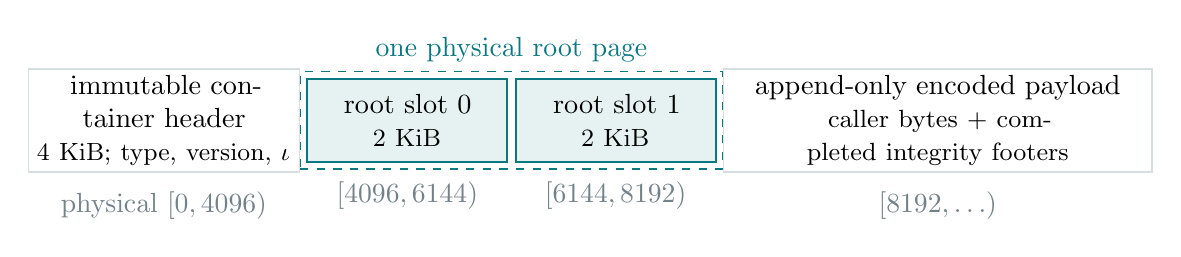
\begin{tikzpicture}[x=1cm,y=1cm]
  \node[box,text width=3.2cm,minimum height=1.05cm] (h) {immutable container header\\\small 4 KiB; type, version, $\inc$};
  \node[root,text width=2.3cm,minimum height=1.05cm,right=.08cm of h] (s0) {root slot 0\\\small 2 KiB};
  \node[root,text width=2.3cm,minimum height=1.05cm,right=.08cm of s0] (s1) {root slot 1\\\small 2 KiB};
  \node[box,text width=5.2cm,minimum height=1.05cm,right=.08cm of s1] (p) {append-only encoded payload\\\small caller bytes + completed integrity footers};
  \node[below=.12cm of h,align=center,text=Muted] {physical $[0,4096)$};
  \node[below=.12cm of s0,align=center,text=Muted] {$[4096,6144)$};
  \node[below=.12cm of s1,align=center,text=Muted] {$[6144,8192)$};
  \node[below=.12cm of p,align=center,text=Muted] {$[8192,\ldots)$};
  \node[draw=Accent,dashed,fit=(s0)(s1),inner sep=.08cm,label={[text=Accent]above:one physical root page}] {};
\end{tikzpicture}
\caption{Filesystem geometry. At the generic wrapper boundary, backing logical offset zero is
physical offset 4096, so the root page and payload are accessed only through ordinary \code{Blob}
methods.}
\label{fig:layout}
\end{figure*}

All root metadata uses the virtual filesystem coordinates in Figure~\ref{fig:layout}. Selecting
encoded payload length $L$ therefore requires physical file length $8192+L$. At the ordinary
backing-\code{Blob} boundary, the immutable 4 KiB container header is hidden, so the corresponding
logical length is $4096+L$ and payload offset $o$ maps to backing offset $4096+o$. Every
$\mathsf{truncate}$ in this paper means this translated full-file length, never the bare payload
length $L$; it cannot remove either the container header or root page.

Generation $g$ occupies slot $g\bmod 2$. Consequently, writing generation $g+1$ cannot overwrite
the slot that contains generation $g$.

\begin{invariant}[Consecutive nonwrapping slot lineage]\label{i:lineage}
Every admitted transition from selected generation $g$ proposes exactly $h=g+1<2^{64}$ and targets
slot $h\bmod2$. Before the first byte of that transition is issued, the target slot's only
barrier-established source image is the all-zero bootstrap image when $h\le2$, or a canonical image
of exactly generation $h-2$. An attempt whose rejection completes consumes $h$ with an exact abort
authority rather than reusing it; provisional rejection enables no reuse. No path skips a
generation or wraps the counter. A blob at generation
$2^{64}-1$ is read-only until migrated to a future format.
\end{invariant}

\subsection{Root header}

\begin{definition}[Canonical empty predecessor]\label{def:zero}
An all-zero 112-byte root-header region in slot zero makes $\Zero_0$ available as the fallback:
generation zero, zero encoded length, unbound integrity, zero tag, and empty payload. It is an
implicit predecessor, not an encoded root header, witness, or group certificate. Ordinary recovery
selects it only when neither slot contains a recoverable ordinary root and no valid later-generation
or wrong-parity root makes zero fallback ambiguous. The first candidate is generation one in slot
one, so arbitrary rejected first-generation bytes in slot one do not alter the untouched
$\Zero_0$ authority in slot zero.
\end{definition}

Every nonzero slot spelling begins with the 112-byte root header in Table~\ref{tab:root}. Unused bytes remain
available for a batch witness. Integers are big-endian.

\begin{table*}[t]
\centering
\small
\begin{tabularx}{\textwidth}{@{}r r l X@{}}
\toprule
Offset & Bytes & Field & Meaning \\
\midrule
0   & 8  & spelling & seven-byte R14 prefix plus one generation-colored state byte \\
8   & 8  & generation & nonzero monotonically increasing generation \\
16  & 8  & encoded length & selected payload length, including completed integrity footers \\
24  & 8  & unfinished start & start of the only unfinished integrity unit \\
32  & 4  & unfinished CRC32C & rolling CRC of the unfinished unit; zero when closed \\
36  & 4  & integrity scheme & 0 unbound, 1 variable, 2 fixed-size chunked \\
40  & 4  & chunk width & nonzero only for fixed-size chunked integrity \\
44  & 64 & application tag & caller-owned state published with this root \\
108 & 4  & root CRC32C & domain-separated CRC over bytes 0--107 \\
\bottomrule
\end{tabularx}
\caption{The root header. The checksum domain is
\code{\_COMMONWARE\_RUNTIME\_ATOMIC\_LOG\_ROOT}.}
\label{tab:root}
\end{table*}

Let
\[
  \Sigma=\{\mathsf{P},\Prepared,\Root,\Abort,\Materialized,\Tombstone\}
\]
and fix
\[
  (\sigma(\mathsf{P}),\sigma(\Prepared),\sigma(\Root),\sigma(\Abort),
    \sigma(\Materialized),\sigma(\Tombstone))
    =(0,1,2,3,4,5).
\]
For nonzero generation $g$ and
state $s\in\Sigma$, define the one-byte transition guard
\[
  \chi(g,s)=1+6(g\bmod 3)+\sigma(s).
\]
The root spelling is the seven ASCII bytes \code{CWUNO14} followed by $\chi(g,s)$.  Thus the state
and the generation color occupy one addressed byte; they are deliberately not two separate fields
that a torn write could splice. Assumption~\ref{a:fault} chooses that byte as old or newly issued,
not as independently torn bits. A decoder cross-checks the color against the encoded 64-bit
generation before checking the root CRC32C.

Let $D_{\mathrm{root}}$ be the ASCII checksum-domain string in Table~\ref{tab:root}. The proposed
R14 fixture stores, in big-endian order,
$\operatorname{CRC32C}(D_{\mathrm{root}}\mathbin\Vert\text{header}[0..108))$ at offsets 108--111.
There is no intervening length or separator. This pins the representative byte vectors used by the
executable model; it does not describe the checked-in R13 root codec as R14.

The root states are:
\begin{center}
\small
\begin{tabularx}{\columnwidth}{@{}c l X@{}}
\toprule
Symbol & State & Ordinary visibility \\
\midrule
$\Root$ & direct committed root & visible independent root \\
$\mathsf{P}$ & direct prepare & invisible direct prepare \\
$\Prepared$ & batch prepare & invisible batch prepare \\
$\Abort$ & rejected-generation authority & visible predecessor-equivalent root \\
$\Materialized$ & retained final root & visible independent retained root \\
$\Tombstone$ & removed final root & namespace deletion marker \\
\bottomrule
\end{tabularx}
\end{center}
The remainder calls the batch-prepared state $\Prepared$; earlier diagrams labeled the same
abstract state ``P.'' Ordinary root recovery recognizes $\Zero_0$, canonical independent
$\Root$, $\Abort$, and $\Materialized$.
$\mathsf{P}$ and $\Prepared$ are deliberately invisible; $\Tombstone$ is interpreted by namespace
recovery rather than exposed as a blob.

\begin{invariant}[Generation-colored provenance]\label{i:color}
Suppose generation $h$ is being introduced into one slot.  Before a decision, the only
generation-$h$ guard bytes that the protocol may issue to that slot are $\chi(h,\Prepared)$ (or
$\chi(h,\mathsf{P})$ for a direct publication) and, during consumption after provisional
rejection, $\chi(h,\Abort)$. It never
issues $\chi(h,\Root)$, $\chi(h,\Materialized)$, or $\chi(h,\Tombstone)$ before their respective
  commit guards. By Invariant~\ref{i:lineage}, every byte already present from the preceding use of
  that slot has color $(h-2)\bmod 3$, which differs from $h\bmod3$. Therefore an arbitrary subset of old, prepared, and
  abort writes cannot contain the guard byte required by an unissued committed or final root.
\end{invariant}

\begin{invariant}[Prepare code-last publication]\label{i:prepareorder}
For R14-2P, phase 1 issues the candidate payload bytes and any required extending length update,
never a decision-dependent shrink, and every byte of
the exact canonical 2 KiB candidate slot except root offset 7. A successful file barrier must cover
those updates and every stamp-specific payload credit on which the candidate depends before live
$\mathsf{BodyReady}_i$ credit is granted. Phase 2 begins only after every participant in $G$ has
live body credit. It is the only transition that may issue $\chi(h,\Prepared)$: it addresses only
offset 7, is enabled by that group-wide live phase-1 join, and has its own durability completion
$\mathsf{GuardDone}_i$. Any crash clears all such live credits. The lifecycle model separately
retains a recovery-inert history bit recording that a guard synchronization once succeeded; this is
proof bookkeeping for acknowledgement, not live $\mathsf{GuardDone}_i$ credit or a recovery input. Recovery has
no transition that writes a $B$ guard and never reconstructs $\mathsf{BodyReady}_i$ from a
guardless body. Consequently, any exact generation-$h$ $B$ observed on disk descends from a
phase-2 issue whose exact same-candidate non-guard slot bytes, wrapped witness, payload, and length
evidence were already durable.
\end{invariant}

\begin{invariant}[Abort code-last publication]\label{i:abortorder}
The write that can place $\chi(h,\Abort)$ is issued only after a successful barrier has made every
other byte of the exact predecessor-equivalent $A_h(O)$ header durable. Until a later authority is
durable, any exact $A_h$ selected by recovery therefore has logical projection $O$; no torn abort
may validate with candidate metadata. A failed or canceled first or second phase returns no mutable
handle and admits no later slot or payload reuse.
\end{invariant}

Before the guard barrier establishes exact $A_h$, the abort body has no rollback authority. After
every crash in either phase, recovery first decodes the entire resulting disk image again. If
already-issued candidate or final evidence remains complete, recovery follows the decision path
rather than resuming rollback; it never writes a missing $B$. Exact $A_h$ has precedence over the stale same-slot witness and is the first
disk state that makes the old classification permanent.

\subsection{Witness wrapper and local link}

A $\Prepared$ slot appends a 16-byte wrapper immediately after the root: 8-byte magic
\code{CWUNOW13}, 4-byte link length, and a 4-byte CRC32C over the wrapper prefix and link under
domain \code{\_COMMONWARE\_RUNTIME\_ATOMIC\_BATCH\_WITNESS}. Up to 1920 link bytes fit in the slot.

Every prepare that introduces a generation has one canonical complete 2 KiB target image. A direct
prepare is $P$ followed by zeros. A batch target image is $B$, its exact wrapper and link, then
zeros through the end of the slot. R14-2P does not issue that image as one unordered overwrite:
phase 1 writes all 2,047 bytes except the guard at root offset 7, and phase 2 writes that one byte
only after phase 1 and the payload/length obligation are durable. Direct finalization changes the
header to $R$ and leaves the zero suffix; group finalization changes only the header to $M/T$ and
preserves the exact witness and zero padding. Completed rejection changes only the header to exact
$A$ and leaves any stale witness physically present but semantically suppressed. This canonical
full-slot grammar is recovery metadata: bytes outside a shorter write are not silently treated as
harmless padding.

Each local link stores the fields in Table~\ref{tab:link}. The containing filesystem path supplies
the local key; only the successor key is encoded. Thus every path appears once around the ring,
not $n$ times in a global descriptor.

\begin{table*}[t]
\centering
\small
\begin{tabularx}{\textwidth}{@{}l r X@{}}
\toprule
Field & Bytes & Constraint \\
\midrule
link magic & 8 & \code{CWUNOL14} \\
group identifier & 16 & fresh $\gid$ \\
participant count, ordinal, flags & 12 & nonzero $n\le 2^{32}-1$; $0\le i<n$; only removal bit defined \\
local incarnation & 16 & equals immutable header incarnation \\
base generation, candidate slot offset & 16 & candidate is generation base$+1$ in the parity slot \\
exact $\Prepared$ and $\Root$ headers & 224 & two complete 112-byte candidate spellings \\
payload validation descriptor & 20 & offset, length, CRC32C; zero length means preflushed/no suffix \\
successor partition length + bytes & $4+|q'|$ & valid partition string \\
successor name length + bytes & $4+|x'|$ & raw name bytes \\
successor incarnation & 16 & exact physical generation expected at the successor path \\
\midrule
fixed portion & 336 & leaves $1920-336=1584$ bytes for one successor partition/name pair \\
\bottomrule
\end{tabularx}
\caption{Local successor link. Names are bounded per edge; they are never summed across the
group into one descriptor.}
\label{tab:link}
\end{table*}

\begin{limitation}[R14-1P witness-splicing negative control]\label{l:witness-provenance}
R14-1P is the former one-phase control that writes the generation-colored $B$ guard, adjacent
generation-independent \code{CWUNOW13} wrapper, and remaining slot bytes in one unordered
full-slot update. Generation coloring proves that a state byte for generation $h$ was issued, but
under that ordering it does not prove that the adjacent witness bytes came from the same prepare.
The wrapper CRC proves byte consistency, not issuance provenance. Under Assumption~\ref{a:fault},
checksum bytes may themselves be selected independently from the old and new slot images.

A concrete protocol-reachable trace starts with an independently finalized generation-one
two-member group $H=\{a,b\}$ and an independent generation-one singleton at $c$, whose length-four
witnesses remain in the same-parity slots. Each
participant then selects an exact empty generation-two ordinary $R$ after rewind, and the
generation-three group $G=\{a,b,c\}$ is a legal four-byte append from that authority. Thus its
links name base generation two and no transition skips a generation; the generation-one slots are
only the older physical witness source. A crash before
any $G$ R14-1P prepare barrier may retain exact issued $B_3$ roots and new candidate fields at $a$ and $b$
while retaining $H$'s group identifier, count, ordinals, and $a\leftrightarrow b$ successor fields.
The wrapper checksums can also be exact old/new mosaics: in one independently reconstructed fixture,
the old/new/hybrid CRC32C values are \code{47ad25a0}/\code{c3bcb36c}/\code{47ad256c} at $a$ and
\code{73a8b16e}/\code{47775580}/\code{7377b16e} at $b$. Each hybrid checksum byte comes from the
old or issued-new checksum at that address and equals the canonical checksum of the hybrid link.
This is exact reconstruction, not a CRC collision. Retaining no generation-three update at $c$
then lets recovery accept a synthetic exact two-member ring, publish $a$ and $b$, and leave $c$
old. The observation of the admitted $G$ is mixed. R14-1P is therefore nonconforming for the
admitted-window guarantee even though its root guard is generation-colored.

R14-2P is the selected noncryptographic repair. Before its phase-1 barrier, no $B_h$ guard has been
issued. After that barrier, every decision-relevant non-guard slot byte, wrapper/link byte,
checksum byte, padding byte, payload byte, and length update for the candidate is exact and durable.
Only then may phase 2 address $\chi(h,\Prepared)$. Thus an observed exact $B_h$ is itself the
disk-visible proof that its canonical witness and payload evidence were established first; no
external witness-intent premise is needed. A crash discards the live phase credit, and recovery
may finalize an already proved ring or publish $A$ code-last, but never writes $B$. A one-layer
design would instead require a root-to-witness commitment over every decision-relevant topology
byte and an explicit computational \emph{splice-binding} assumption; CRC32C or ordinary collision
resistance is insufficient. That alternative is not the reference protocol. The checked-in R13
format remains a separate generation-uncolored negative control and is not made conforming by this
selection.
\end{limitation}

\begin{definition}[Candidate]
A candidate $c_i$ is the tuple
\[
  (g_i-1,o_i,B_i,R_i,a_i,\ell_i,z_i),
\]
where $g_i$ is the proposed generation, $o_i$ its parity slot, $B_i$ and $R_i$ are the exact
$\Prepared$ and $\Root$ headers, and $(a_i,\ell_i,z_i)$ describes the speculative payload suffix.
The two headers must agree in every field except spelling and root checksum.
\end{definition}

\begin{definition}[Canonical integrity geometry]\label{def:integrity}
For root fields $(L,u,c,s,w)$ and encoded payload $V[0..L)$, write
$\mathsf{IntegrityOK}(L,u,c,s,w,V)$ when all of the following hold:
\begin{enumerate}
  \item $0\le u\le L$; the unfinished bytes are exactly $V[u..L)$; $c$ is their rolling CRC32C,
  with the canonical value zero when $u=L$.
  \item Unbound is encoded only as $(s,w)=(0,0)$ and requires $u=0$. It has no completed units.
  \item Variable integrity is encoded only as $(s,w)=(1,0)$. The prefix $V[0..u)$ is a
  concatenation of caller-delimited nonempty data units, each followed by its four-byte big-endian
  CRC32C footer; $V[u..L)$ is the one possibly empty unfinished unit.
  \item Fixed integrity is encoded as $(s,w)=(2,N)$ for $1\le N\le 2^{32}-1$.
  The prefix length $u$ is a multiple of $N+4$ and consists of exact $N$-byte data units followed
  by four-byte big-endian CRC32C footers; its unfinished tail satisfies $L-u<N$.
\end{enumerate}
Ordinary root open checks the numeric scheme, bound, alignment, and closed-checksum conditions
without scanning completed payload. Footer and rolling-CRC equality are construction invariants and
are validated when the corresponding integrity unit or tail is read.
\end{definition}

\begin{definition}[Eligible candidate]\label{def:eligible}
$\mathsf{Eligible}(c_i)$ holds only if the candidate has generation exactly one above its base,
does not wrap, occupies the parity-selected slot, satisfies Invariant~\ref{i:lineage}'s exact
same-slot source condition, has a canonical root encoding, and would pass ordinary root recovery at
the candidate encoded length. $\mathsf{IntegrityOK}$ holds and the issued physical
payload covers that encoded length. Every candidate payload byte must be exactly one of:
\begin{enumerate}
  \item an unchanged byte selected by the predecessor root;
  \item a current stamped value covered by preflush durability credit; or
  \item a current stamped value in the candidate's one exact contiguous speculative suffix, whose
  descriptor ends at the candidate length and carries its CRC32C.
\end{enumerate}
A prepare transition may issue no candidate for which this predicate or the aggregate suffix bound
is false.
\end{definition}

\begin{definition}[Allowed torn transition]
Let $X_i$ be the 112 bytes currently read from candidate slot $o_i$. For a retained participant,
\[
  \begin{aligned}
    \mathcal{S}_{i,j} &= \{B_i[j],R_i[j],A_i[j],M_i[j]\}, \\
    \mathsf{Transition}(X_i,c_i) &\iff \forall j,\;X_i[j]\in\mathcal{S}_{i,j}.
  \end{aligned}
\]
For a removed participant, $T_i[j]$ is also admitted. Here $A_i$ is the predecessor-equivalent
abort root, while $M_i$ and $T_i$ are deterministically derived from $R_i$ by changing the
generation-colored spelling and recomputing the root checksum. Byte membership alone is not a
decision predicate: recovery also requires the guard byte to name a state whose write was enabled
by the transition system. Invariants~\ref{i:color} and~\ref{i:prepareorder} make both the state
issue and the exact candidate-body/witness provenance of a $B$ guard disk-observable.
\end{definition}

Recovery applies exact-$A_i$ precedence before using this predicate as candidate evidence. Exact
$A_i$ is included in the allowed byte set so interrupted repair images can be classified, but an
exact abort root suppresses its same-slot witness and cannot participate in a deciding ring. For a
non-$A$ image, the wrapper and link must themselves validate exactly. Installation overwrites only
the first 112 bytes, so the already durable witness remains available even when the final root write tears.
The appearance of $R_i$ in $\mathsf{Transition}$ makes its byte values legal during repair; it does
\emph{not} make an ordinary root proof of this group.

For final installation, recovery uses the stronger predicate
\[
  \mathsf{FinalTransition}_i(X,F) \iff
  \left(\forall j,\;X[j]\in\{B_i[j],F_i[j]\}\right)
  \land \left(X=B_i\ \lor\ \exists j,\;F_i[j]\ne B_i[j]\land X[j]=F_i[j]\right),
\]
where $F_i$ is the canonical $M_i$ or $T_i$ target. The successful phase-2 barrier established
exact $B_i$ as the durable base before any final write was enabled. No other write to those 112
bytes intervenes. Therefore $X=B_i$ retains the prepared ring, while $X\ne B_i$ contains at least
one target-only byte whose persistence proves that the final write was issued after
$\mathsf{decide}(G)$. This discriminator includes a root-checksum byte even when the $B$ guard
survives. Byte membership without this exact-base condition is not final-decision evidence.

\begin{definition}[Group-bound final certificate]\label{def:certificate}
A final certificate for participant $i$ of $G$ is the pair consisting of (a) the exact candidate
$M_i$ spelling for a retained participant or $T_i$ for a removed participant and (b) the adjacent
exact wrapped witness naming $G$, $i$, and $c_i$. An exact $R_i$ is not a group certificate because
the root header contains no group identifier.
\end{definition}

\begin{definition}[Abort authority]\label{def:rollback-fence}
Let authority at generation $g$ select logical state $O_i$, and let its opposite slot contain a
rejected candidate or an orphaned partial transition for generation $h=g+1$.  The abort authority
$A_i=\Abort_h(O_i)$ is a canonical 112-byte root header with guard $\chi(h,\Abort)$ and with every
logical field copied from $O_i$.  It consumes generation $h$ without changing the logical
projection.  Recovery gives an exact $A_i$ precedence over any same-slot witness; the stale witness
may remain physically present but has no authority.

Abort publication is code-last. First, while leaving the one-byte spelling guard unaddressed,
recovery writes the other 111 root bytes of $A_i$---including the checksum computed for the final
$A_i$ spelling---and crosses a file barrier. Then it writes only $\chi(h,\Abort)$ and crosses a
second barrier. Before the first barrier, no $A$ guard exists. After it, every non-guard byte is the
exact predecessor-equivalent $A_i$ value. A crash during the one-byte second phase therefore leaves
either the prior non-$A$ guard or the complete exact $A_i$; it cannot combine an $A$ guard with a
candidate-valued body. On the live path, an abort authority is established only after the second
barrier succeeds. If that barrier is interrupted, the open generation is poisoned; after a crash,
recovery may accept a complete exact $A_i$ that happened to land, or repeat the two phases from the
partial image. It never relies on the pre-crash process having observed success.
\end{definition}

\begin{definition}[Canonical and quiescent slot]\label{def:quiescent}
A complete slot image is canonical exactly when it is one of: (a) the all-zero unused image;
(b) an exact $P_h$ or $R_h$ header followed only by zeros; (c) an exact $B_h$, $M_h$, or $T_h$
header followed by its exact same-generation wrapped link and zeros after the declared link; or
(d) an exact $A_h$ header, whose ignored suffix may retain the rejected witness. After
recovery has selected authority at generation $g$, its opposite-parity slot is
$g$-\emph{quiescent} only when it is all zero or is a canonical image of generation $h<g$.
Every other opposite-slot byte string is an orphaned partial transition, even if no root or wrapper
inside it validates. An exact canonical image with generation at least $g$ is resolved before this
predicate is evaluated; it is not classified as inactive.
\end{definition}

\section{Logical protocol state}

\subsection{Per-blob state}\label{sec:blob-state}

The selected protocol state of one blob is
\[
  S=(g,L,u,c,s,w,t,V[0..L)),
\]
comprising internal generation, encoded length, unfinished-integrity start and CRC, integrity scheme
and width, 64-byte caller tag, and the exact encoded payload bytes selected below $L$. Its logical
projection is
\[
  \pi(S)=(L,u,c,s,w,t,V[0..L)),
\]
which omits the protocol generation. Payload content is part of the logical value even though it is
not repeated in the root. The in-memory state may
additionally contain an unpublished append tail or a shorter staged length.

For $g=0$, $S$ is the canonical $\Zero_0$ state of Definition~\ref{def:zero}; for $g>0$, it is
selected by a checksummed root spelling.

For proof purposes each issued payload byte carries a monotonically fresh write stamp. A durability
credit is a triple $(o,v,e)$ saying that a successful file barrier covered value $v$ written at
offset $o$ with stamp $e$. Credit belongs to that exact value and stamp, not merely to the offset.
Rewind invalidates every credit at or above the new physical end before those offsets may be reused;
replacement appends receive new stamps. A concurrent preflush credits only the snapshot of issued
stamps ordered before its barrier. This is the abstract counterpart of the implementation's payload
checksum/frontier tracker.

Appends issue payload writes immediately; UNO does not retain the complete epoch in memory. A
rewind below the selected length fences later appends until the shorter root is durable, after
which the backing file may be truncated in place. If a crash loses that physical truncate, root
recovery repeats it before the discarded offsets are reused. Regardless of whether the physical
truncate survived, replacement bytes remain uncovered until their own exact stamps are synced or
included in the candidate's validated suffix.

Protocol-owned payload integrity is orthogonal to batch publication. A completed caller-delimited
or fixed-size unit has one 4-byte CRC32C footer. The selected root stores the start and rolling CRC
of the only unfinished unit. Ordinary independent-root recovery reads neither completed payload nor
the unfinished unit; validation occurs only when that unit is requested. Namespace recovery of an
unresolved group may additionally stream its bounded speculative suffix before choosing a root.

\subsection{Groups and the canonical ring}

After duplicate elimination and conflict checks, participants are sorted strictly by key:
\[
  \keyof(p_0)<\keyof(p_1)<\cdots<\keyof(p_{n-1}).
\]
Link $i$ declares ordinal $i$, count $n$, and successor
$p_{(i+1)\bmod n}$. Every link carries the same fresh group identifier $\gid$. Removal is a local
bit and is also reconstructed as a sorted subset of participants.

The same canonical order is used for participant locking, ordinals, successor validation, and
descending deletion. Caller order therefore cannot create a distinct ring or opposing lock order.

\begin{invariant}[Exact closed ring]\label{i:ring}
A ring is complete only if following successors for exactly $n$ steps finds: one unique matching
witness at each exact key/incarnation; the same $\gid$ and $n$; consecutive ordinals modulo $n$;
strictly increasing keys after rotation to ordinal zero; pairwise-distinct current device/inode
identities; and closure to the starting exact incarnation on step $n$, neither earlier nor later.
\end{invariant}

\begin{invariant}[No ring contraction]\label{i:nocontraction}
A candidate that declares group identifier $\gid$ and count $n$ can authorize only that exact
$n$-participant ring. A missing, suppressed, replaced, malformed, or early-closing successor never
causes recovery to reinterpret the reachable participants as a smaller group. In particular, a
surviving participant is not a singleton merely because no peer remains reachable; a one-participant
decision must have been admitted with count one and an exact self-link. An independent $M/T$
certificate may bypass traversal after decision, but it proves the earlier $n$-participant decision
and does not construct a smaller ring.
\end{invariant}

\begin{figure*}[t]
\centering
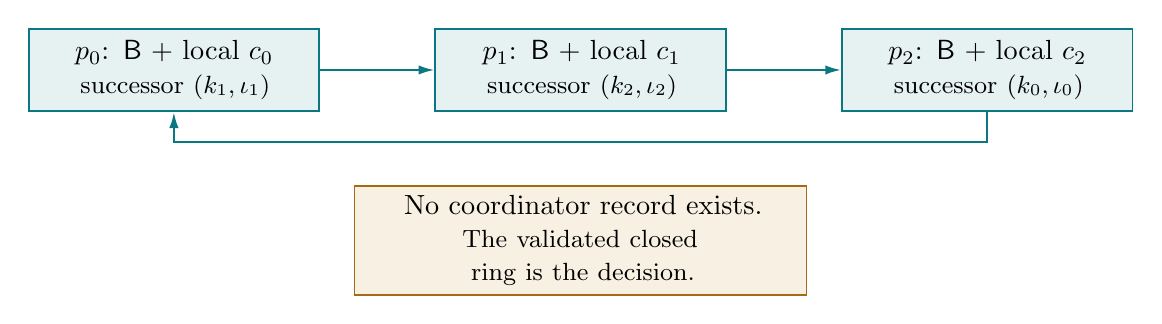
\begin{tikzpicture}[node distance=1.45cm]
  \node[root,text width=3.45cm,minimum height=1.05cm] (a) {$p_0$: $\Prepared$ + local $c_0$\\\small successor $(k_1,\inc_1)$};
  \node[root,text width=3.45cm,minimum height=1.05cm,right=of a] (b) {$p_1$: $\Prepared$ + local $c_1$\\\small successor $(k_2,\inc_2)$};
  \node[root,text width=3.45cm,minimum height=1.05cm,right=of b] (c) {$p_2$: $\Prepared$ + local $c_2$\\\small successor $(k_0,\inc_0)$};
  \draw[flow] (a) -- (b);
  \draw[flow] (b) -- (c);
  \draw[flow] (c.south) -- ++(0,-.38cm) -| (a.south);
  \node[warn,below=.92cm of b,text width=5.5cm] {No coordinator record exists.\\\small The validated closed ring is the decision.};
\end{tikzpicture}
\caption{Three participants linked in canonical order, closing on the exact starting incarnation.
A one-participant publication self-links.}
\label{fig:ring}
\end{figure*}

\section{Transition system}\label{sec:transitions}

A configuration contains the namespace map, each inode's two raw slots and payload bytes, the
durable base and post-barrier updates from Assumption~\ref{a:fault}, and volatile lock/carried-group
state, including per-participant $\mathsf{BodyReady}$ and $\mathsf{GuardDone}$ credits. A crash
clears both credits before recovery begins. An abstract proof-history bit may remember that a
guard synchronization returned successfully, but recovery neither reads that bit nor treats it as
durable disk evidence. An initial configuration contains only durably and
directly named regular-file participants whose two slots are
canonical, whose selected roots or canonical $\Zero_0$ predecessors and payloads pass ordinary
recovery, and whose logical-key-to-inode map is injective with canonical integrity geometry; it
contains no unsuppressed prepared witness. A configuration is
\emph{protocol-reachable} iff it follows from an initial configuration by the guarded transitions
below, an allowed crash, and any prefix of recovery. These rules are normative: a backend that can
produce another transition does not refine this protocol.

\begin{description}
  \item[Stage payload.] Append writes encoded bytes once at their final offsets without changing a
  selected root. Preflush may establish stamp-specific durability credit. A rewind below the
  selected length must become a selected durable root before an append may reuse discarded offsets;
  it invalidates all old credit for those offsets. No offset named by a rejected candidate may be
  truncated, overwritten, or reused while that candidate could still be rediscovered as an exact
  ring; the abort-authority transition below must run first.

  \item[Prepare $G$, phase 1: body and evidence.] While all keys in $K_G$ are exclusively locked,
  validate exact current directly named regular files, incarnations, and pairwise-distinct current
  device/inode identities, construct only $\mathsf{Eligible}$ candidates, and establish
  Invariant~\ref{i:payload}. Issuing the first non-guard slot byte is $\mathsf{admit}(G)$; payload
  staging alone remains invisible. For each participant, issue its required candidate
  payload and extending-length updates (never a rewind shrink) and write all 2,047 bytes of the canonical
  $B_i$/wrapped-link/zero-padding slot except root offset 7. Leave that guard byte unaddressed. A
  successful file barrier covering this exact body and every payload credit grants volatile
  $\mathsf{BodyReady}_i$. A phase-1-only image is not a prepare vote.

  \item[Prepare $G$, phase 2: code-last $B$ guard.] Only after live
  $\mathsf{BodyReady}_j$ exists for every $j\in G$ may normal execution issue any one-byte
  $\chi(g_i,\Prepared)$ write at root offset 7. No other byte is addressed in this phase. Its
  separate successful durability completion grants $\mathsf{GuardDone}_i$. The group-wide body
  credit remains live only for this phase-2 attempt and is cleared after the join, an error, or a
  crash. Recovery contains neither phase-1 continuation nor a $B$ writer: it
  re-decodes disk and chooses finalization or code-last $A$ normalization. No prepared root is an
  ordinary visible root.

  \item[Normal decision and acknowledgement.] Phase-1 obligations may run concurrently across
  participants, but the join of every phase-1 completion precedes every phase-2 guard issue.
  Phase-2 obligations may then run concurrently. Only the successful join over \emph{all}
  phase-2 guard durability completions establishes $\mathsf{decide}(G)$ on the live path; only then
  may $\mathsf{ack}(G)$ occur. There is no protocol order among participants within either layer.

  \item[Recovery decision.] If no live join exists, recovery may establish
  $\mathsf{decide}(G)$ only after excluding exact $A$ at every candidate generation, then reading
  one exact closed ring whose nonfinal anchors carry exact $B$ guards, checking every
  $\mathsf{Transition}(X_i,c_i)$ and $\mathsf{Eligible}(c_i)$, and validating all non-preflushed
  payload suffixes. Invariant~\ref{i:prepareorder} derives each accepted witness's provenance from
  that $B$ issue; recovery consults no witness-intent oracle. After finalization begins, an anchor
  may instead carry $\mathsf{FinalTransition}$ evidence relative to its exact durable $B$ base; an
  unchanged $B$ or any target-only final byte preserves the same disk-derived decision. A
  group-bound final certificate is itself disk-derived proof that this validation or the normal
  join occurred earlier; selecting that local final state does not require a traversable witness
  chain. Traversal from such a certificate repairs reachable nonfinal peers. Traversal remains
  mandatory when nonfinal $B$/link evidence is instead used as the collective decision proof.
  Within protocol reachability, a broken ring at a final anchor means the unreachable participants
  already have independent-final roots or serialized later authorities. A guardless phase-1 body,
  missing path, incomplete link, ordinary $R_i$, or malformed candidate is never a prepare vote.

  \item[Provisional rejection and consumption.] If the current disk image does not prove a
  candidate reached through an exact wrapped witness, recovery first resolves the predecessor
  authority. If that predecessor is a carried linked decision, recovery makes it group-wide
  independently final before suppressing any of its links. Recovery then attempts to publish $A_i$
  from Definition~\ref{def:rollback-fence} code-last into one required witness slot: synchronize the
  111 non-guard bytes, then synchronize the one-byte $A$ guard. The initial rejection is not durable
  authority. After any crash or uncertain barrier, recovery re-reads every root, witness, and
  required payload byte before continuing. If the disk still proves an already-issued complete
  candidate or final transition, it establishes $\mathsf{decide}(G)$ and finalizes new. If exact $A_i$ is
  present, it suppresses the stale witness and selects old. Only after predecessor finalization and
  exact $A_i$ may recovery return a mutable handle or permit a candidate payload offset to be
  truncated, overwritten, or reused. The exact abort root consumes the candidate generation while
  preserving the old logical value; its generation-colored guard is distinct from every unissued
  $R/M/T$ guard for that generation. Recovery never promotes a guardless phase-1 body by writing
  $B$; $A$ is its only prepare-slot guard writer.

  \item[Normalize an orphaned slot.] After recovery resolves every exact higher-generation root,
  final certificate, and wrapped candidate, it evaluates Definition~\ref{def:quiescent} from the
  selected generation $g$. If the opposite slot is not $g$-quiescent, recovery treats it as an
  unrecognizable partial transition. It first makes any linked selected authority group-wide
  independently final, then publishes $A_{g+1}$ code-last into the opposite slot. No wrapper is required
  to enter this branch. Recovery may return a mutable handle, truncate or reuse payload, or use the
  other slot for the next generation only after the abort-root barrier succeeds. A crash during
  normalization restarts the complete byte-derived classification, including candidate and payload
  evidence that may have survived a partial abort body; it never relies on memory that the abort
  write had once begun.

  \item[Finalize.] Only after $\mathsf{decide}(G)$ may recovery or normal execution issue $M_i$ for
  retained participants and $T_i$ for removals. Each repair attempt is an ordinary fallible write
  followed by a file barrier and may be interrupted at any byte subset. The next recovery
  reclassifies that partial image before retrying. Group-wide independent finalization holds only
  after \emph{every} participant's final write has succeeded or an exact final image has been
  recovered from a crash; until then all original witnesses remain intact. For each torn peer,
  $\mathsf{FinalTransition}$ yields either its unchanged exact $B$ root or a target-only persistent
  byte proving the post-decision final write. The complete set of witnesses and these per-root
  classifications repair the group even during the first final write.

  \item[Unlink.] No participant path may be unlinked before group-wide independent finalization.
  Cleanup may target only a removed participant after revalidating its exact key, incarnation,
  witness, tombstone, and currently named inode. It then synchronizes the parent directory. A
  missing or replaced path is left untouched.

  \item[Proof transfer and slot reuse.] A witness required to recover $G$ may be overwritten,
  suppressed, or made unreachable only after either (a) group-wide independent finalization of
  $G$, or (b) a complete, $B$-proven decision for a consecutive group over exactly the same ordered
  keys/incarnations has become durable in the alternate slots. A phase-1-only successor cannot
  suppress the predecessor. Case (b) transfers the serial prefix to the successor ring; if the
  successor is incomplete, the predecessor ring remains intact. Any
  other overlapping operation---including an abort root that would suppress a linked
  predecessor---first takes route (a). Before a direct $\mathsf{P}\to R$ publisher may prepare a
  slot containing rejected evidence, recovery must consume that rejected generation with the same
  abort authority; the direct publication then uses the next parity slot. Merely invalidating a few
  wrapper bytes and reusing the rejected generation is outside the transition system. An ordinary
  $R$ is never group evidence.

  \item[Conflicting non-group mutation.] Create, direct publish/rewind, exact remove, and
  whole-partition remove acquire the same logical-key/namespace exclusion as groups. Before their
  admission, every decided carried group touching a target key is made group-wide independently
  final; these operations are not exact-ring successor transfers. Create first resolves any
  tombstone, then installs a fresh named inode generation and satisfies
  Assumption~\ref{a:admission} before returning a batch-eligible handle. Direct publication uses its
  own invisible prepare and durable independent root, including the proof-transfer and abort-authority guards
  above. Remove first resolves touching witnesses, then unlinks only the exact current target,
  synchronizes every affected directory, and invalidates its live generation while retaining
  namespace exclusion. A whole-partition remove applies that rule to every contained key. A crash
  before admission leaves selected states unchanged; after admission, the operation follows its
  ordinary API recovery semantics and every surviving effect is serialized after the finalized
  groups it touched. UNO makes no new atomicity claim for whole-partition removal itself.

  \item[Recovery selection.] Candidate rings are considered by descending generation. Any newer
  exact independent $R$, $A$, $M$, or $T$ state at a key suppresses older witnesses at that key;
  $A$ selects its predecessor-equivalent value and $T$ maps the key to logical absence. An exact
  local group-bound $M/T$ certificate is selected before ring
  traversal and is never rolled back merely because a deletion has broken its successors. For the
  newest remaining prepared candidate, recovery either rejects an incomplete ring or guardless
  phase-1 body with no certificate provisionally and begins abort publication, or establishes the
  decision and finalizes the whole group. Before a provisionally rejected candidate's
  predecessor becomes mutable, an exact code-last $A$ has made the old classification durable. If neither an exact
  candidate nor a newer authority is recognizable, the orphan-normalization transition resolves
  every non-quiescent opposite slot before mutability. It never exposes $B$ directly and never
  writes a $B$ guard. Recovery transitions obey
  the same finalization, unlink, and proof-transfer guards and may themselves crash.
\end{description}

The rules separate an evidence predicate from a historical event. In particular, a final
certificate proves $\mathsf{decide}(G)$, not necessarily that the original pre-crash sync calls
returned: recovery itself may first validate a fully surviving unacknowledged ring and then issue
the certificate.

\section{Normal execution}

\subsection{Preparation}

The namespace owner performs the following steps while conflicting namespace and participant
mutations are excluded.

\begin{lstlisting}[style=protocol,caption={Prepare one group $G$.}]
canonicalize operations by (partition, raw name)
validate current handles, exact incarnations, rewinds, and names
reject symbolic-link entries
reject repeated device/inode identities under distinct keys
for each dirty participant i:
    derive candidate (B_i, R_i) for generation g_i + 1
    choose the bounded payload suffix not already durable
    if suffix is ineligible or exceeds its assigned recovery share:
        sync the current immutable payload; then use an empty suffix
require every candidate to satisfy Eligible(c_i)
choose fresh group id gamma
encode one canonical full slot: B_i || wrapper(link_i) || zero padding
preflight every link against its 1,920-byte local capacity
for every participant i, concurrently where possible:
    issue candidate payload/extension, if any
    write every candidate-slot byte except root offset 7
    sync participant i                    // phase-1 durability
    set live BodyReady_i
\end{lstlisting}

Pending payload can be arbitrarily large subject to address-space, file, and implementation
limits. Background preflush may run while appends continue. The current backends divide the
64 MiB recovery budget among locked mutations, which may preflush a large participant even when the
aggregate suffix would fit. The protocol requires only the resulting aggregate bound. Preflush
changes no visible root and never rewrites payload.

\begin{invariant}[Payload coverage]\label{i:payload}
For every candidate whose ring can still establish or repair a decision (that is, it has not been
durably consumed by $A$ or suppressed by a newer authority), each payload byte below its suffix start either
is an unchanged byte selected
by the predecessor root or has stamp-specific durability credit from a successful file barrier
before the $\Prepared$ guard write is issued. The remaining exact contiguous suffix ends at the
candidate length and is either empty or described by a CRC32C over its current stamped values.
Across one group, nonempty suffix lengths sum to at most 64 MiB. Rewind and offset reuse cannot
reuse credit belonging to an earlier value.
\end{invariant}

\subsection{Decision round}

Phase 1 has already made the exact non-guard slot body, wrapped local link, candidate payload, and
length evidence durable. A deletion candidate names the last committed length, not discarded
pending bytes. Phase 2 writes only the prepared guard at offset 7 and completes a second per-file
durability operation. The obligations within either layer may run concurrently through a runtime
backend; the protocol does not depend on any particular kernel submission interface or on physical
flush coalescing.

\begin{lstlisting}[style=protocol,caption={Establish and acknowledge a decision.}]
require live BodyReady_j for every participant j
for every participant i, concurrently where possible:
    write candidate_slot_i[7] := chi(g_i, B)  // one byte only
    sync participant i                         // phase-2 durability
    set live GuardDone_i
wait until every participant GuardDone_i is established
clear all live phase credit
record the complete decision in process memory
return Ok from start_apply       // durable acknowledgement
\end{lstlisting}

There is no later coordinator write. If acknowledgement occurred, both layers and all covered
payload are durable. If an earlier crash leaves an incomplete set of $B$ guards, recovery chooses
old through code-last $A$ normalization; a complete exact $B$-proven ring chooses new. The
R14-1P control does not have this dichotomy: Limitation~\ref{l:witness-provenance} shows that one
unordered slot write can reconstruct a complete synthetic ring over only a strict subset of the
admitted participants.

\begin{invariant}[Prepared invisibility]\label{i:invisible}
No $\Prepared$ root is selected by ordinary blob recovery. Until namespace recovery validates an
entire group, each participant's preceding $\Zero_0$, $\Root$, $\Abort$, $\Materialized$, or
complete predecessor-ring proof remains its only visible authority.
\end{invariant}

\begin{invariant}[Rejected-candidate generation consumption]\label{i:retirement}
If recovery has completed rejection of a candidate group and has made its predecessor available for mutation,
then any collective predecessor proof was made group-wide independently final before that first
availability, and one required rejected-ring slot contains a durable exact $A$ root at the rejected
generation. Until exact $A$ is established, candidate payload ranges
remain immutable and no truncate or offset reuse may be admitted. By parity, the abort-root slot
cannot be addressed again before a strictly higher-generation authority exists in the alternate
slot, so future arbitrary-subset rewrites cannot restore the old group's authority.
\end{invariant}

\begin{invariant}[Staggered rejection and later mutation]\label{i:staggered}
After exact $A_i$ has durably consumed participant $i$'s candidate for rejected group $G$, normal
mutation guards may admit a later operation at $i$ without first normalizing every unresolved peer
of $G$. Such a peer remains non-mutable until its own recovery either finds independent final
evidence, validates a complete exact ring, proves that no distinguishable candidate-generation
effect remains, or durably consumes its distinguishable candidate with its own
predecessor-equivalent $A$. A newer authority, missing successor, or replaced incarnation at
$i$ can only break traversal of $G$; it cannot contract $G$ or make a peer's prepared candidate
visible. This staggered permission applies only to a rejected group. If $\mathsf{decide}(G)$ was
established, a later operation over a different participant set remains blocked by
Invariant~\ref{i:reuse} until every participant of $G$ has an independent final root.
\end{invariant}

\begin{invariant}[Mutable-return slot normalization]\label{i:normalize}
Recovery returns a mutable handle selecting generation $g$ only if the opposite slot is
$g$-quiescent, or after a durable $A_{g+1}$ has advanced the selected authority without changing
its logical projection. A failed or canceled normalization returns no handle. This guard applies
even when neither a root nor a wrapper in the opposite slot validates.
\end{invariant}

\subsection{Materialization and activation}

After the decision, a retained candidate can be rewritten as independently recoverable
$\Materialized$; a removed candidate becomes a payload-preserving $\Tombstone$. Each rewrite is a
112-byte write followed by a file barrier, and may itself be interrupted at any addressed-byte
subset. A live repair counts as durable only after that barrier succeeds; a post-crash exact root is
reclassified from disk. The exact $M/T$ header together with its exact adjacent witness is a
group-bound final certificate. An ordinary $\Root$ is never such a certificate. Normal execution
issues no final rewrite until every phase-2 guard durability completion has joined; recovery may do
so after independently validating a complete ring and its payload.

The certificate claim depends on Invariants~\ref{i:color} and~\ref{i:prepareorder}, not merely on
CRC validation. Code-last $B$ first binds the exact witness to the admitted candidate. Before
$\mathsf{decide}(G)$, no transition writes $\chi(g_i,\Materialized)$ or
$\chi(g_i,\Tombstone)$ into candidate slot $i$. Old same-parity state has a different color, and
the $B/A$ state bytes for generation $g_i$ are distinct. Therefore an exact $M/T$ spelling cannot
be assembled by a torn prepare or abort write before the guarded final write is issued.

Removal-free groups may remain in the linked state and be carried in process memory. A following
group with exactly the same participant keys/incarnations and consecutive generations may use the
other slots and supersede it directly; that successor may itself contain a removal and will then be
eagerly finalized. A different participant set or any conflicting namespace operation first
materializes the carried decision group-wide.

\begin{invariant}[Proof transfer before reuse]\label{i:reuse}
A witness needed to recover a decided group is not removed, overwritten, or suppressed unless
either (a) \emph{every} participant in that group has a durable independent final root, or (b) a
consecutive group over the exact same participant ring has established a complete durable successor
decision in the alternate slots.
\end{invariant}

\subsection{Deletion}

Deletion uses the following normal completion sequence:
\begin{enumerate}
  \item durably write $\Materialized$ for every retained participant and $\Tombstone$ for every
  removed participant;
  \item wait for \emph{all} final-root writes to succeed;
  \item visit removed participants in descending canonical ordinal;
  \item for each one, verify exact key/incarnation, witness, tombstone, and current inode; unlink;
  then synchronize its parent directory before moving to the next lower ordinal.
\end{enumerate}

\begin{invariant}[Final-before-unlink]\label{i:finalfirst}
No path is unlinked on behalf of group $G$ until every participant of $G$ has a durable independent
final root.
\end{invariant}

Define $\mathsf{IndependentFinalized}(G)$ to mean that every retained participant has an exact
durable $\Materialized$ root, every removed participant has an exact durable $\Tombstone$, and the
durable local witness remains beside each spelling. Each record then determines that participant's
new logical state without traversing the ring.

\begin{invariant}[Independent authority before unlink]\label{i:independent}
If an unlink on behalf of $G$ is enabled or has been issued, then
$\mathsf{IndependentFinalized}(G)$ was established before the first such unlink. Until admission
of a later mutation touching a key in $K_G$, each retained participant remains independently
$\Materialized$, while each removal is represented by its exact $\Tombstone$ or by the missing name
produced from that tombstone. After such an admission, any replacement authority is produced by the
serialized later transition and denotes a state ordered after $G$, never a state before $G$.
\end{invariant}

\begin{invariant}[Tombstone dominance]\label{i:tdominance}
Once namespace recovery identifies an exact current-incarnation $\Tombstone$, that incarnation is
logically absent and remains so unless a serialized create installs a fresh named generation.
Exact-name open may report absence or perform that create, and scan must omit the tombstoned
incarnation; neither path may fall through to any older ordinary or linked authority in the
alternate slot.
\end{invariant}

\begin{invariant}[Incarnation-safe cleanup]\label{i:cleanup}
Cleanup may unlink a path only after validating the expected participant incarnation, exact
$\Tombstone$, wrapped witness, and currently named inode. A missing path or a different
incarnation is never removed on behalf of the old decision.
\end{invariant}

Descending ordinal order and a directory barrier after each unlink give the common crash path a
cheap, resumable frontier. They are a reclamation policy, not a safety dependency after
Invariant~\ref{i:independent} holds. A later exact-name open may remove one surviving tombstone, and
a partition scan may remove several and synchronize the directory once. Such out-of-order cleanup
can break the ring and strand other physical tombstones, but it cannot change their logical state.

\section{Recovery}

Recovery has two layers. Namespace recovery first resolves linked decisions and deletions. Only
then does ordinary per-blob recovery choose the newest valid $\Root$, predecessor-equivalent
$\Abort$, or $\Materialized$ root, or the canonical $\Zero_0$ fallback, and truncate any physical
surplus to the selected length. Namespace recovery interprets an exact current-incarnation
$\Tombstone$ as absence before ordinary fallback selection.

\subsection{Discovering a ring}

Opening one atomic participant inspects its two witness wrappers. For each intact wrapper, recovery
decodes the local link and follows exactly its declared count. At each successor it:
\begin{enumerate}
  \item opens the exact path without following symlinks;
  \item validates the immutable container header and required incarnation;
  \item resolves every strictly higher-generation recognizable candidate, exact independent
  $R/A/M/T$ authority, or non-quiescent raw slot before accepting an older witness, and gives an
  exact same-generation $A$ precedence over its adjacent witness;
  \item searches the two slots for exactly one witness matching group, count, expected ordinal,
  candidate slot, and local incarnation; and
  \item verifies the candidate transition and exact wrapped witness, and requires an exact $B$
  guard for an undecided nonfinal candidate. A generation-colored final guard is considered only
  on the post-decision transition path described below.
\end{enumerate}
Missing, duplicated, ambiguous, early-closing, out-of-order, stale-incarnation, overlong, malformed,
guardless, or non-closing paths provisionally reject a prepared candidate only when the anchor lacks an exact group-bound
final certificate. An exact local $M/T$ certificate is examined before traversal because legitimate
deletion may already have broken the ring. Recovery never scans unrelated names.

After all recognizable candidates and authorities have been resolved, recovery also inspects each
complete raw slot image. If the inactive slot fails Definition~\ref{def:quiescent}, it cannot be
silently ignored: it is normalized through the same abort authority before a mutable
handle or payload reuse is permitted. This branch is deliberately independent of wrapper validity.

\begin{lstlisting}[style=protocol,caption={Recover from one intact witness.}]
if anchor has a strictly newer recognizable candidate or non-quiescent raw slot:
    ResolveNewerGeneration(anchor)
    restart recovery selection
if anchor has a strictly newer exact independent R/A/M/T authority:
    SelectNewerIndependentAuthorityOrAbsence(anchor)
    return NEWER
if anchor slot contains exact A for this candidate generation:
    SelectPredecessorEquivalentAbort(anchor)
    return OLD                    // exact A suppresses the stale witness
if anchor has an exact group-bound final certificate M/T:
    links := TryFollowExactlyNLinks(anchor)
    if links form one exact canonical closed ring:
        FinishDecision(links)     // repair any still-linked peers
    else:
        SelectIndependentFinal(anchor)
        TryOrderedDeleteCleanup(anchor)
    return FINAL
links := FollowExactlyNLinks(anchor)
if links do not form one exact canonical closed ring:
    IndependentlyFinalizeLinkedPredecessorIfAny()
    PublishAbortRoot(anchor, predecessor logical value)
    return OLD only after exact A is durable
if any peer has an exact group-bound final certificate M/T:
    FinishDecision(links)         // decision was already durable
else if every participant has exact B and every candidate and suffix validates:
    FinishDecision(links)         // complete code-last prepare survived
else if every root is exact B or a valid final transition
        and at least one target-only final byte survived:
    FinishDecision(links)         // exact-B base plus target byte proves earlier decision
else:
    IndependentlyFinalizeLinkedPredecessorIfAny()
    PublishAbortRoot(anchor, predecessor logical value)
    return OLD only after exact A is durable
authority := select the preceding visible or carried authority at generation g
if opposite raw slot is not g-quiescent:
    IndependentlyFinalizeLinkedAuthorityIfAny(authority)
    PublishAbortRoot(g + 1, logical_value(authority))
    restart recovery selection
return authority only after the mutable-return normalization guard
\end{lstlisting}

The exact-$B$ branch derives witness provenance from disk: phase 2 could address that guard only
after the same candidate's phase-1 body, wrapper, payload, and length evidence crossed a barrier.
A guardless phase-1 body is never promoted. A final target-only byte is also ordered after a
decision: the exact $B$ durable base precedes every final write, and no other transition intervenes
at those addresses. Invariant~\ref{i:color} separately prevents exact pre-decision synthesis of an
$M/T$ guard. Recovery never invokes either prepare phase and contains no $B$ write.

The broken-ring certificate branch never rolls back or aborts the final anchor. Within protocol
reachability, a ring can become broken after an exact local final certificate only after the
final-before-unlink guard made every participant independently final, or after a serialized later
mutation. The anchor therefore selects its own new state while peers select their $M/T$, missing,
or later authorities.

The abort root is required for every admitted guardless or incomplete candidate whose stale witness
or payload descriptor remains distinguishable. Otherwise a later rollback and append could reuse
offsets that the stale witness treats as preflushed, and a
second crash could make the old suffix validate against a payload prefix that old group never
proposed. Merely zeroing or complementing witness bytes is insufficient: successive partial slot
rewrites could reconstruct an older byte pattern. The generation-consuming $A$ root avoids that
ABA shape without rewriting the witness. Making a linked predecessor independent first preserves
its group-wide authority when the newer abort root suppresses its ring witness. The pre-$A$
validation failure is not itself durable authority; exact $A$, not that failed validation, makes
the old outcome monotone without retaining in-memory write stamps on disk.

A crash during abort publication does not create an undocumented fourth case. The next recovery
first reruns the ordinary disk predicates. It may recognize already-issued complete candidate or
final evidence and decide new; recognize complete $A$ and select old; or see a noncanonical raw
slot and repeat normalization. It never installs a missing $B$. If the torn image happens to equal an older canonical
quiescent image,
then no distinguishing byte of the rejected higher-generation image remains in the recovered
durable base; it is safe to reuse under the validity event in Assumption~\ref{a:trusted}. In
particular, while introducing generation $g+1$, the guard byte can come only from the older
same-slot color, $\chi(g+1,\Prepared)$, or $\chi(g+1,\Abort)$. It cannot equal an unissued
$\chi(g+1,\Root)$, $\chi(g+1,\Materialized)$, or $\chi(g+1,\Tombstone)$. No branch depends on
remembering that a pre-crash process intended to write $A$.

If both slots contain recoverable linked candidates, they are considered by descending generation.
A later exact independent $\Root$, $\Abort$, $\Materialized$, \emph{or} $\Tombstone$ suppresses
stale witnesses. This permits exact-ring supersession while preventing replay of an old group over
a newer predecessor-equivalent value, retained value, or deletion. Same-generation $R$ cannot
certify a stale ring: it is either
separated from batch use by the direct-publication retirement guard or is a protocol violation.

\subsection{Arbitrary torn final roots}

The final $\Materialized$ or $\Tombstone$ write may tear at any subset of its 112 addresses. The
root CRC may consequently be invalid. Recovery does not need to guess a prefix boundary: the exact
candidate witness supplies the canonical $B$ and $M/T$ values, and
$\mathsf{FinalTransition}$ checks every byte independently. Immediately before the first final
write, every $B$ root and witness is exact and durable. If no target-only byte survives, that root
is still exact $B$; otherwise the surviving target-only byte proves the post-decision write was
issued even when the state guard remains $B$. Recovery therefore does not require a second exact
certificate to repair the first torn final root. Every retry can tear again; only a successful
barrier or a later recovered exact spelling advances that participant to independent final state.

This repair is safe only because the R14-2P phase-1 barrier made the witness durable before the
$B$ guard could establish a decision, and final installation writes do not overlap it. If a medium
may damage unwritten neighboring bytes, Assumption~\ref{a:fault} does not hold.

\subsection{Recovery with missing participants}

A missing successor observation does not have one generic meaning. Recovery distinguishes missing
candidate evidence at a still-present participant, same-group unlink after finalization, a later
serialized unlink or replacement, and external loss of a retained path. None of these observations
is itself a prepare vote.

\paragraph{Incomplete candidate with a retained participant.}
If the expected path/incarnation remains but its exact $B$ guard, wrapped link, candidate transition,
or required payload evidence is absent, the ring is incomplete and supplies no authority. If one
participant's phase-1 body/evidence failed to cross its barrier, Invariant~\ref{i:prepareorder}
forbids issuing a $B$ guard anywhere. After the group-wide phase-1 join, every body is durable, but a
crash may retain only a proper subset of the separately issued phase-2 guards. Both cuts choose old
unless already-issued final evidence proves a decision. No missing $B$ is reconstructed by
recovery, and no remaining predecessor becomes mutable until the required distinguishable rejected
generation is consumed by exact $A$.

\paragraph{Pre-finalization missing path during the protected interval.}
If following a prepared ring encounters a missing exact path before any group-bound $M/T$
certificate is known, the ring is likewise incomplete; a missing blob whose local removal bit would
have been set is \emph{not} evidence that the batch committed. Before admission of a later serialized
conflicting mutation, the path cannot have been removed by UNO because UNO issues no unlink on
behalf of this group before finalization. An actual missing path in that interval is external
namespace interference or corruption and may fail closed rather than fabricate a complete old
vector. After that interval, an authorized later mutation may itself remove the path; the serialized
case below applies and the absence still supplies no vote for this group.

\paragraph{Staggered rejection after successor advancement.}
Let incomplete group $G$ declare the ring $a\to b\to c\to a$, with no group-bound final
certificate and with $b$ lacking required candidate evidence. Opening $a$ fails exact traversal at
$b$, resolves any linked predecessor, and publishes exact $A_a$ before returning $O_a$ for
mutation. A later singleton or different-set operation $H$ may then advance $a$ through one or more
generations. When $c$ is opened later, its surviving link still declares $G$ and count three. Its
wrap edge finds $A_a$ or a newer authority at $a$, not the exact matching $G$ witness. Recovery does
not need the old generation at $a$, does not reinterpret $c$ as a singleton, and does not scan for
an alternate route. In the absence of local final evidence or a complete exact ring, it resolves
its preserved predecessor, publishes exact $A_c$, and returns $O_c$. The resulting history is the
rejection of $G$ followed by $H$.

The corresponding decided history is deliberately different. If $\mathsf{decide}(G)$ had been
established, $H$ could not suppress $a$'s witness as a different-set operation until proof transfer
had installed independent final roots at every participant, including $M_c$ for retained $c$ (or
$T_c$ before an authorized removal). A later open of retained $c$ would select that local final
certificate before traversal. Thus an unresolved prepared root at $c$ together with an advanced
successor cannot be a protocol-reachable decided-and-suppressed history.

\paragraph{Deletion broke a finalized ring.}
After unlinks start, the full ring may no longer be traversable even though the decision is already
durable. This is safe because the first unlink is downstream of independent final roots at every
participant. Present $\Materialized$ roots select new retained values, and present $\Tombstone$
roots independently denote logical absence. Before any later mutation of a key in $K_G$, a
protocol-generated missing path can only be a removed participant: cleanup for $G$ never unlinks a
retained participant. A later operation may replace or remove a retained incarnation only after
Invariant~\ref{i:reuse} has made $G$ independently recoverable; that later operation is ordered
after $G$ and is outside Definition~\ref{def:atomic}'s observation interval.

For example, let decided group $G$ declare $a\to b\to c\to d\to a$ and remove $b$ and $d$.
Before either unlink, exact $M_a,T_b,M_c,T_d$ are all durable. Once $b$ and $d$ are absent, the
surviving links at $a$ and $c$ may each point directly into a hole, so no surviving ring component
connects them. They nevertheless remain members of the original four-participant decision: $M_a$
and $M_c$ select their new values independently, without traversal and without treating either
participant as a singleton. If a later operation advances $a$ before $c$ is opened, $c$ still
selects $M_c$; the recovered serial history contains $G$ followed by the later operation at $a$.
Protocol-reachable failure to reach $a$, $b$, or $d$ after those tombstone unlinks or that later
serialized operation does not strand $c$.

\paragraph{Hole created by a later serialized operation.}
A later operation may remove or replace a participant only after the older decided group is
independently final or an allowed exact-ring successor has transferred its proof. If the older group
was rejected instead, the later operation resolves the rejected evidence on every key it touches,
while a durable abort authority keeps that old outcome irreversible for still-unopened peers. A
later hole therefore contributes only a later serialized namespace effect. It never authorizes the
older group, contracts its participant count, or makes a prepared survivor independently visible.

The implementation still attempts the following eager reclamation walk when ordinal zero survives:

\begin{lstlisting}[style=protocol,caption={Recover an ordered delete frontier from ordinal zero.}]
require exact final candidate and witness at ordinal 0
prefix := []
for expected ordinal j = 1 .. n-1:
    append current exact final link to prefix
    if exact successor path/incarnation is unavailable:
        dirsync(parent(next))     // persist observed frontier
        for link in reverse(prefix):
            if link.removed:
                verify T; unlink; dirsync(parent)
        return COMMITTED
    require successor has exact M or T and expected link j
    current := successor
reject a non-closing intact chain here; full-ring recovery handles it
\end{lstlisting}

On the normal descending path, a missing exact successor or a path with a replacement incarnation
ends forward traversal. After re-synchronizing that successor's parent directory, the implementation
may reclaim the already verified lower prefix in reverse order. The exact final ordinal-zero
certificate and group-wide independent roots authorize that cleanup; the hole or replacement is
never itself a commit vote. A non-prefix hole therefore limits discovery but does not make verified
prefix cleanup unsafe. Logical recovery relies on Invariants~\ref{i:independent}
and~\ref{i:tdominance}; if the parent directory itself is absent, the current availability
deviation in \S\ref{sec:implementation-status} applies.

An exact-name open that finds a current-incarnation tombstone first reports the old incarnation
absent, unlinks the lingering name, and may then create a fresh named inode generation. Atomic open
mints a fresh V2 incarnation; ordinary open may create a non-atomic V1 blob. A partition scan applies the same
test to every canonical file, unlinks every confirmed tombstone, then synchronizes the partition
directory once. Consequently no surviving tombstone is returned as live even if the ring or the
descending frontier is no longer traversable. Tombstones that are neither opened nor encountered
by a scan may remain allocated indefinitely; this is delayed reclamation, not logical resurrection.

\begin{limitation}[Externally missing retained participant]\label{l:externalmissing}
The missing-path argument relies on exclusive namespace ownership. On behalf of a group, UNO
unlinks only exact tombstones, so before a later serialized mutation of that key, a missing retained
participant is not protocol-reachable after independent finalization. A later authorized remove may
make the retained incarnation absent, but that effect is ordered after the group. A file removed by
another process or lost independently by the medium is corruption outside the conditional
crash-atomicity target; UNO does not reconstruct its payload or promise failover semantics.
\end{limitation}

\subsection{Recreation and stale paths}

When a deleted key is recreated atomically, its new 128-bit incarnation differs. An ordinary V1
replacement has no matching V2 incarnation. Ring traversal therefore rejects either as the expected
participant. Stale cleanup also compares the inode opened for validation with the inode currently
named at the path immediately before unlink. Thus a replay of an old tombstone cannot remove a
replacement that reuses the same human-readable name.

\section{Safety argument}

All results in this section are conditional on Assumptions~\ref{a:fault}--\ref{a:identity}.
``Valid'' means checksums do not collide. The invariants are consequences of the guarded transition
system rather than additional assumptions. For the normative R14-2P system,
Invariant~\ref{i:prepareorder} derives the provenance of every accepted $B$ witness from protocol
ordering; witness issuance is not an external theorem premise. Limitation~\ref{l:witness-provenance}
shows why the same conclusion is false for the R14-1P negative control. The result below remains a
conjecture because the current executable obligations are pending and, even if completed, are
bounded and decomposed; the production and filesystem refinement obligations also remain open.

\begin{lemma}[Invariant preservation]\label{lem:preservation}
Every protocol-reachable configuration satisfies Invariants~\ref{i:color}, \ref{i:prepareorder}, \ref{i:abortorder},
  \ref{i:lineage}, \ref{i:ring}, \ref{i:nocontraction}, \ref{i:payload},
\ref{i:invisible}, \ref{i:retirement}, \ref{i:staggered}, \ref{i:normalize}, \ref{i:reuse},
\ref{i:finalfirst}, \ref{i:independent}, \ref{i:tdominance}, and~\ref{i:cleanup}.
\end{lemma}
\begin{proof}
Induct on transitions from the initial configuration. Stage-payload steps do not change a selected
root; their stamp rule invalidates credit on rewind/reuse and grants credit only after a barrier.
Every admitted root or candidate transition proposes exactly the consecutive generation in the
opposite slot. Rejection consumes that generation with $A$, no transition reuses it, and the maximum
generation admits no successor, preserving Invariant~\ref{i:lineage}.
Prepare admits only eligible candidates and constructs one canonical exact ring. Its first phase
issues candidate payload/length updates and every non-guard slot byte, and grants
$\mathsf{BodyReady}_i$ only after a successful barrier establishes the exact body, witness, and
payload evidence. Its second phase begins only after the group-wide body-credit join, addresses
only the $B$ guards, and records separate guard durability completions. A crash may tear either
issued update but clears all live phase credits. Before the body barrier no $B$ was issued; after it, any issued $B$ names the
already durable exact candidate. Recovery contains no $B$ writer, so induction across restarts
cannot promote a guardless body. Initial-state injectivity, alias rejection, conforming creation,
and exclusive namespace ownership preserve distinct participant inodes. A crash cannot invent an
unissued generation-colored state byte or alter the alternate slot; $B$ remains invisible to
ordinary root selection. Traversal never rewrites decoded group identity, count, ordinal, or
successor fields: any mismatch rejects the candidate, while local $M/T$ selection uses a final
certificate rather than constructing a smaller ring.
Reject-and-consume first applies the ordinary group-wide finalization guard to any linked
predecessor, then establishes all non-guard $A_i$ bytes before issuing its state guard. Thus an
exact $A_i$ has the predecessor projection even if either phase crashes. Parity leaves $A_i$
untouched until a higher-generation authority exists in the alternate slot, so later partial
rewrites cannot make the consumed generation selectable again. Before exact $A_i$, however, the
classification remains provisional. A crash during abort publication returns no handle; canonical
slot decoding first re-evaluates complete candidate and payload evidence, then either decides new,
selects exact $A_i$ as old, or classifies the raw opposite slot as non-quiescent and retries
normalization. The same byte-derived guard covers a partial transition whose wrapper no longer
validates. Establishing a decision changes only a monotone fact; failure to establish it does not.
After exact $A_i$, later operations at $i$ preserve suppression of the rejected ring, while each
unresolved peer retains its predecessor and remains subject to its own mutable-return normalization.
Finalize is guarded by the positive decision fact and starts from the barrier-established exact
$B$ root. It preserves the non-overlapping exact witness. Thus every crash image is either unchanged
$B$ or carries a target-only byte in $\mathsf{FinalTransition}$, and recovery rederives rather than
remembers the decision. Finalization reaches group-wide independence only after every $M/T$ write
succeeds. Unlink is guarded by group-wide independence and exact incarnation/witness/inode checks.
Proof transfer permits witness retirement only after group-wide independence or a complete,
  $B$-proven same-ring successor decision in the alternate slots. Recovery uses the same guards, prioritizes
  newer $R/A/M/T$ authority, treats every surviving exact $T$ as absence, and may crash back into the
same induction. These are all transitions in Section~\ref{sec:transitions}.
\end{proof}

\begin{lemma}[Alternating-slot predecessor preservation]\label{lem:fallback}
Issuing candidate generation $g+1$ cannot overwrite the slot record for generation $g$.
\end{lemma}
\begin{proof}
Slots are selected by generation parity. Consecutive generations have opposite parity. Under the
addressed-write model, the candidate write can alter only its own 2 KiB slot, so the prior slot is
unchanged. The phase-1 body and phase-2 guard address only that parity-selected slot. For $g=0$,
generation one uses slot one and leaves slot zero's all-zero root-header
fallback. For
$g>0$, the prior record is either an independent root or the complete linked proof carried from the
immediately preceding exact-ring group.
\end{proof}

\begin{lemma}[Abort-authority permanence]\label{lem:rollback}
Once $A_i$ for rejected group $G$ is durable, no later protocol-reachable crash image can use
participant $i$ as the exact witness required to select $G$.
\end{lemma}
\begin{proof}
Immediately after the barrier, the candidate slot contains a valid independent root at $G$'s local
generation whose logical projection is the predecessor. The old witness bytes may remain, but
same-slot $A$ has recovery precedence over them. Payload writes do not address the slot. By
alternating parity, the next
root or witness update for this participant uses the other slot. Before any protocol transition may
reuse the abort-root slot, that intervening generation has become an independent root or a complete
durable linked decision; it is strictly newer than $G$ and suppresses $G$ under recovery selection.
This suppression is established before the reused-slot write is issued, so it survives every
arbitrary subset of that write and every later crash. Thus bytewise mixtures may reconstruct old
bytes physically, but they cannot restore $G$'s authority.
\end{proof}

\begin{lemma}[Disk-derived orphan normalization]\label{lem:normalize}
A crash during candidate preparation, candidate rejection, or abort-root publication cannot
make recovery return the predecessor for mutation while an unrecognized higher-generation slot
remains reusable.
\end{lemma}
\begin{proof}
Recovery first resolves every exact root, certificate, and wrapped candidate. If none applies, it
compares the complete opposite slot against the canonical grammar in
Definition~\ref{def:quiescent}. A noncanonical image enables no mutable return and is overwritten by
another code-last $A_{g+1}$ attempt. A crash during that attempt restarts this classification; if
the new image still proves already-issued candidate or final evidence, recovery decides new rather
than assuming the earlier rejection remains valid. A guardless phase-1 prepare body is such a noncanonical image, not
a latent permission to issue $B$: its pre-crash $\mathsf{BodyReady}$ credit was lost and recovery
has no $B$ transition. During the first phase of abort publication the $A$ guard is absent; during its
second phase all other $A$ bytes are already barrier-established. Hence an exact $A_{g+1}$ is a
newer independent authority with the
same logical projection. An exact higher candidate is processed normally. An all-zero or strict
lower-generation canonical image contains no unsuppressed higher-generation protocol record in the
recovered durable base. If generation $g+1$ remains distinguishable, Invariant~\ref{i:color}
limits its guard byte to the prepared/direct-prepare state or the abort state until a commit guard
actually issues another state. Thus no torn normalization can synthesize a new visible or final
authority. Every path that permits mutation has
either removed the orphan from the durable base or placed it behind a newer authority. Repeating
the argument after each crash establishes the claim without volatile intent state.
\end{proof}

\begin{lemma}[Incomplete prepare is invisible]\label{lem:incomplete}
If a candidate ring is missing any exact $B$ guard, exact link, eligible candidate transition, or
required payload byte, and no post-decision final evidence exists, recovery does not expose any
candidate state from that ring.
\end{lemma}
\begin{proof}
Ring traversal requires all $n$ exact participants and closure by Invariant~\ref{i:ring}. Missing,
guardless, or malformed state provisionally rejects the ring in the current image. A structurally
complete ring additionally validates every candidate and its payload suffix. Failure is also
provisional. Recovery cannot fill a missing $B$ guard: Invariant~\ref{i:prepareorder} clears the
only enabling credit on crash and gives recovery no such writer. By
Invariant~\ref{i:invisible}, $\Prepared$ is not selectable by ordinary recovery. By
Lemma~\ref{lem:fallback} and the group-wide form of Invariant~\ref{i:reuse}, either the preceding
canonical $\Zero_0$, independent root, or complete predecessor-ring proof remains recoverable from
the alternate slots. Before that predecessor is returned for mutation,
Invariant~\ref{i:retirement} requires an exact independent abort root unless the complete candidate
slot has reverted byte-for-byte to its canonical lower-generation pre-attempt source. That source
may contain its own exact lower-generation witness; the exceptional image retains no distinguishing
  byte or witness effect from the admitted candidate generation. If an intervening crash leaves an
  already-issued complete candidate recognizable, Lemma~\ref{lem:complete} applies and recovery
  selects the whole new vector. Otherwise, before any participant is returned for mutation, exact
  $A$ consumes that participant's distinguishable rejected generation; unresolved peers remain
  non-mutable until their own recovery performs the same classification and, when required,
normalization. Only then do Lemmas~\ref{lem:normalize} and~\ref{lem:rollback} permit offset reuse
at that participant without reviving the candidate. Thus the incomplete candidate is invisible in
every individual image, while the pre-$A$ rejection classification itself need not be monotone.
\end{proof}

\begin{lemma}[Staggered peer recovery]\label{lem:staggered}
Let incomplete group $G$ have no group-bound final evidence, and let exact $A_i$ durably reject its
candidate at participant $i$. Protocol-reachable later operations at $i$ cannot strand an unresolved
participant $j$, make $j$ accept a strict subset of $G$, or require $j$ to recover the superseded
generation at $i$.
\end{lemma}
\begin{proof}
Lemma~\ref{lem:rollback} makes $i$ permanently unusable as the exact witness required by $G$; every
later exact authority at $i$ preserves that suppression before the abort slot can be reused. When
$j$ later follows its surviving $G$ link, the missing or nonmatching successor therefore fails the
exact $n$-member predicate. Invariant~\ref{i:nocontraction} forbids treating the reachable fragment
as a smaller group. Lemma~\ref{lem:fallback} and Invariant~\ref{i:reuse} preserve $j$'s predecessor
as an independent authority or a linked authority that is made independent before suppression.
Recovery can consequently publish predecessor-equivalent $A_j$ and return the old logical value
without reading the old generation at $i$.

The only apparent conflicting history would decide $G$ before the later operation at $i$ while
leaving $j$ merely prepared. That history is outside the transition system: a different-set later
operation cannot suppress a decided witness until Invariant~\ref{i:reuse} has made every participant,
including $j$, independently final. In that case $j$ selects its local $M/T$ certificate before
traversal instead of taking the rejection path.
\end{proof}

\begin{lemma}[Complete prepare is sufficient]\label{lem:complete}
If recovery validates a complete exact-$B$ prepared ring for R14-2P with no group-bound final
certificate, every participant of the admitted $G$ has its candidate state reconstructible in full.
\end{lemma}
\begin{proof}
For each participant, exact $B$ implies that phase 2 issued its guard. By
Invariant~\ref{i:prepareorder}, that issue followed a successful phase-1 barrier over the exact
same-candidate non-guard slot bytes, wrapped link, payload, and length evidence. The fresh group ID,
exact count/ordinal sequence, and canonical closure therefore identify the decoded participant set
and witnesses with the admitted $G$ without an external issuance premise. The ring supplies the
exact candidate root and identity for every participant.
Definition~\ref{def:eligible} validates candidate length, parity, integrity geometry, and ordinary
recoverability. By Invariant~\ref{i:payload}, bytes
before each suffix start were durable before its prepared guard could be issued. Recovery reads
the entire remaining suffix and verifies its exact length and CRC32C. Under the no-collision
assumption, all bytes named by every candidate are therefore present. Rewriting all retained roots
to $\Materialized$ (and removals to $\Tombstone$) cannot synthesize a partial candidate.
\end{proof}

\begin{lemma}[Final certificate implies an established decision]\label{lem:certificate}
An exact group-bound $\Materialized$ or $\Tombstone$ certificate can exist only after
$\mathsf{decide}(G)$ for the same admitted group named by its preserved witness.
\end{lemma}
\begin{proof}
There are exactly two finalize guards. Normal execution first joins successful phase-2 guard
durability completions for every participant. Recovery first validates the complete exact ring, every eligible
candidate, and all required suffix bytes. Either guard establishes $\mathsf{decide}(G)$ before any
$M/T$ byte is issued. By Invariant~\ref{i:color}, neither the older same-slot image, the $B$ prepare,
nor an $A$ abort contains $\chi(g_i,\Materialized)$ or $\chi(g_i,\Tombstone)$. An exact $M/T$
header therefore implies that the corresponding final write was issued; it cannot be an
exact bytewise reconstruction assembled from pre-decision writes. A crash may tear that later
write but cannot reorder its issue event before the decision that enabled it. The final write preserves the adjacent
witness. Its earlier authentic-$B$ preparation is derived from Invariant~\ref{i:prepareorder}, so
the certificate is bound to the admitted $G$; an unbound $R$ is excluded by
Definition~\ref{def:certificate}.
\end{proof}

\begin{lemma}[Installation convergence]\label{lem:install}
Once a group-bound final certificate exists, recovery can make every still-present exact participant
independently final without consulting payload history.
\end{lemma}
\begin{proof}
Lemma~\ref{lem:certificate} establishes the decision predicate, whose two constructors both prove
the candidate payload, so crash-time suffix rehashing is no longer required as a commit test. Each
intact witness names the exact legal root
spellings. The bytewise final-transition predicate accepts any subset tear from the exact durable
$B$ base, distinguishes an unchanged $B$ root from a target-only final byte, and rejects unrelated
bytes. Recovery rewrites the deterministic $\Materialized$ or $\Tombstone$
header durably. Within Definition~\ref{def:atomic}'s observation interval, a protocol-generated missing path
after finalization was an exact tombstone that has already been unlinked; a missing retained
participant is excluded by Limitation~\ref{l:externalmissing}. After that interval, proof transfer
and fresh named-generation identity order any replacement or removal after this group.
\end{proof}

\begin{lemma}[Post-finalization namespace independence]\label{lem:delete}
Once UNO may issue the first unlink, any subset of removed-participant names may subsequently be
absent without changing the group's logical new vector, even when no surviving link reaches another
surviving participant. Cleanup never unlinks a retained participant or a recreated incarnation.
\end{lemma}
\begin{proof}
By Invariants~\ref{i:finalfirst} and~\ref{i:independent}, the first unlink is downstream of an exact
durable final root at every participant. A retained participant is never an unlink target and its
$\Materialized$ root selects the new value independently. For a removed participant, either its
exact $\Tombstone$ remains and Invariant~\ref{i:tdominance} makes it logically absent, or its name is
missing and the same absence is represented physically. Thus arbitrary holes among removed names
cannot create a mixed vector. The surviving links retain their original count and successors; they
are neither required for local $M$ selection nor reinterpreted as smaller rings. Finally,
Invariant~\ref{i:cleanup} requires incarnation, witness, and
inode equality immediately before unlink, so cleanup for the old decision cannot remove a same-name
replacement. Descending traversal only reduces how much garbage later opens or scans must reclaim.
\end{proof}

\begin{lemma}[Composition with later namespace operations]\label{lem:composition}
After independent finalization of group $G$, a later serialized operation may remove or replace any
participant of $G$ and thereby create an arbitrary hole in $G$'s ring without making recovery
observe a state ordered before $G$.
\end{lemma}
\begin{proof}
Invariant~\ref{i:independent} first transfers $G$'s authority from collective ring closure to one
independent final record per participant. A later operation is admitted only after that transfer or
the exact-ring successor transfer allowed by Invariant~\ref{i:reuse}. If it removes a participant,
that effect is ordered after $G$; if it recreates the key, the replacement has a fresh named
generation (and a fresh V2 incarnation when atomic).
Invariant~\ref{i:cleanup} prevents stale cleanup for $G$ from touching that replacement. Every
untouched participant still has its independent $\Materialized$ or $\Tombstone$ state. Therefore a
broken ring changes only which eager cleanup walk is available, and recovery admits the serial
history containing $G$ followed by the later operation.
\end{proof}

\begin{conjecture}[R14-2P group crash atomicity]\label{thm:atomic}
A conforming implementation of the R14-2P transition system satisfies
Definition~\ref{def:atomic}: during $G$'s protected logical-key interval, every protocol-reachable
crash image exposes either $G$'s complete old vector or its complete new vector, never a mixed
vector.
\end{conjecture}
\paragraph{Supporting argument.}
The following case split explains why the preceding invariants support the conjecture; it is not a
machine-checked proof or a refinement proof for the filesystem or implementation.
Lemma~\ref{lem:preservation} supplies the protocol invariants, including the ordering-derived
provenance of every accepted $B$ witness. Partition the trace at the crash into three disjoint cases.

\emph{No pre-crash decision, and recovery returns old without establishing one:} there is no
group-bound final certificate. If every candidate slot equals its canonical lower-generation
pre-attempt source, including any witness belonging to that source, the prepare left no
distinguishable candidate-generation admission effect and the predecessor vector is already
authoritative. Otherwise, every guardless phase-1 or partial phase-2 image before exact $A$ either
lacks complete candidate evidence or is reclassified into the next case. The crash erased every
live prepare credit and recovery cannot write $B$. Lemma~\ref{lem:incomplete} keeps an incomplete
candidate invisible, and no caller mutation, destructive payload change, or slot reuse is enabled
during this provisional interval. Proof-preserving predecessor finalization may still run. Exact
$A$ then selects the complete predecessor vector, changes only internal generation,
and makes that old outcome permanent by Lemma~\ref{lem:rollback}. If a torn abort write destroys the
recognizable witness without producing complete candidate evidence, Lemma~\ref{lem:normalize}
routes the raw non-quiescent slot back through normalization rather than mutable fallback.

\emph{No pre-crash decision, and recovery establishes one before exact $A$:} recovery has found a
complete exact-$B$ ring and validated every candidate and suffix. Code-last ordering identifies
that ring with the admitted group. No recovery write supplied a missing guard.
Lemma~\ref{lem:complete} proves the complete candidate vector, after which finalization yields the
new vector.

\emph{A pre-crash decision exists:} the normal join of all phase-2 guard durability completions or
an earlier recovery already established $\mathsf{decide}(G)$. If no exact group-bound certificate
exists, no unlink is enabled; all paths and exact witnesses remain. For each participant, either the
exact $B$ root remains or $\mathsf{FinalTransition}$ contains a target-only byte relative to that
known durable base. The all-$B$ case reconstructs the complete ring; any other case proves that a
post-decision final write was issued. The preserved witness identifies the same candidate and
payload, so recovery finalizes the group. This covers a crash during the first final write that
leaves no exact $M/T$ spelling and retains only a new checksum byte. If a
certificate exists, Lemmas~\ref{lem:certificate} and~\ref{lem:install} repair every present
participant. If unlink has removed some or all deleted participants, Lemma~\ref{lem:delete} maps
every missing or surviving tombstoned removal to absence while retained $M$ roots select all
retained candidates. This includes an all-removal group with no surviving path.

No unlink is enabled during provisional rejection or on the exact-$A$ old path. On either new path,
the final-before-unlink guard and Lemma~\ref{lem:delete} map every removal to logical absence without
mixing retained participants. Thus these cases exhaust successful recovery traces and yield only
the two vectors in Definition~\ref{def:atomic}.

\begin{remark}[Refinement status]
Conjecture~\ref{thm:atomic} is a manual argument for the normative R14-2P transition system, not a
machine-checked end-to-end theorem, a production-Rust refinement, or an ext4/JBD2 refinement. The
current bounded Kani matrix is pending for its exact 42-harness source snapshot. Completed matrices
for older 30- and 36-harness snapshots checked the three abstraction layers separately and found
the paired R14-1P counterexample in Limitation~\ref{l:witness-provenance}; those results do not
transfer to the current source. The R13 baseline at
\code{26a532dd6} also has
counterexamples to newer-$T$ authority, group-bound certificate selection, rejected-witness reuse,
filesystem namespace ownership, and an ineligible integrity candidate. The reviewed branch repairs
the namespace-ownership item without changing the storage format; the other counterexamples remain.
Current code also relies on, but does not mechanically enforce, the direct-regular-file and no-alias
namespace preconditions. Executable correspondence and each repair obligation are recorded in
\S\ref{sec:implementation-status}.
\end{remark}

\begin{corollary}[Acknowledged durability]\label{cor:ack}
In a conforming implementation, if \code{start\_apply} returns \code{Ok}, every later recovery
returns the new group vector or a state obtained by serializing later protocol-reachable mutations
after that vector.
\end{corollary}
\begin{proof}
Acknowledgement occurs only after every phase-1 body/evidence barrier and every phase-2 guard
durability completion succeeds. Thus the group has a durable byte-for-byte copy of the actually
issued complete ring and $\mathsf{decide}(G)$ even if no root has yet been materialized.
Finalization preserves that witness, and later groups are serialized on overlapping participants
and preserve or transfer the earlier proof before slot reuse. Lemma~\ref{lem:composition} covers
later namespace changes that physically break the earlier ring.
\end{proof}

\begin{limitation}[R14-1P admitted-window failure]\label{l:admitted-window}
If physical admission occurred but \code{start\_apply} did not return \code{Ok}, the current
R14-1P negative control can return a partially new vector. The old-two/new-three trace in
Limitation~\ref{l:witness-provenance} is a concrete counterexample. A validation failure or
cancellation proved to precede admission still leaves only old selected states. This limitation
does not apply to the selected R14-2P transition system; it is retained to prevent the one-phase
control from being mistaken for a conforming optimization.
\end{limitation}

\begin{proposition}[No cross-group temporal order]
For disjoint groups $G$ and $H$, UNO records no durable order between their decisions. If neither
has been acknowledged, a crash may recover either complete group, both, or neither. R14-2P does not
permit a synthetic subset within either group; R14-1P does, as a negative control. An acknowledged
group still satisfies Corollary~\ref{cor:ack} independently.
\end{proposition}
\begin{proof}
Neither ring contains a link, sequence number, or authority belonging to the other. Per-file
barriers impose no cross-file order. Current backends may serialize calls under a process-local
namespace lock, but that scheduling fact is not persisted as protocol state.
\end{proof}

\section{Progress and resource bounds}

\subsection{Recovery work}

Core independent-root recovery reads two fixed root headers and does not scan payload. A public
filesystem open first performs bounded namespace recovery, which may inspect the immutable header
and both full 2 KiB witness slots before selecting those roots. An unresolved group followed from
one anchor visits exactly $n$ declared links and reads at most 64 MiB of speculative payload across
the group. Thus, for total successor-name bytes $K$, one candidate recovery attempt costs
\[
  T_{\mathrm{recover}}=O(n+K+64\,\mathrm{MiB}),\qquad
  M_{\mathrm{recover}}=O(n+K),
\]
independent of historical blob length and the number of prior epochs. The 64 MiB term is a byte
ceiling, not an allocation requirement; validation streams in bounded chunks.
Because one anchor has two slots, an exact-name open may make at most two such candidate attempts,
so its speculative-payload ceiling is 128 MiB in the worst case, still a history-independent
constant. An abort-authority repair may also materialize the immediately preceding linked group, but that
proof is already one of those two slot-local candidates.

A partition scan is not one candidate attempt. Without per-scan group-ID deduplication it may
rediscover the same $n$-member ring from $n$ names, for $O(n^2)$ metadata work and repeated
idempotent final-root writes in the worst case. It remains independent of historical payload size,
but the tighter one-anchor bound must not be attributed to a full scan.

There is no UNO-specific participant policy cap. The on-disk count is a \code{u32}; installation
uses chunks of at most 32 concurrent workers without limiting membership. Each edge independently
limits its successor partition plus name to 1584 bytes.

\subsection{Liveness conditions}

\begin{proposition}[Conditional completion]
For each decided group $G$ unresolved after restart, suppose that after some time crashes and
cancellations cease, required nonremoved paths remain available, a surviving member of $G$ is
eventually inspected, recovery work and lock acquisition are scheduled fairly, and every issued
storage operation eventually succeeds. Then recovery materializes or supersedes $G$. In a live
process, a removal-free decided group may instead remain indefinitely as an active durable carried
ring; that is a completed logical decision, not promised physical materialization. After independent
finalization, logical completion no longer requires an intact ring; physical tombstone reclamation
additionally requires that each lingering name or its partition eventually be inspected.
\end{proposition}

This is not availability under media loss. A missing retained participant, a corrupt immutable
header, a checksum collision, or a permanently failing barrier may prevent completion. The system
fails closed rather than inventing payload. Physical deletion has weaker liveness: a stranded
tombstone whose name is never opened and whose partition is never scanned may consume space
indefinitely, although it remains logically absent.

\subsection{Write and memory cost}

Payload bytes are issued when appended and are not recopied into a transaction log. The abstract
R14-2P steady-state decision adds, per dirty participant, one logical 2,047-byte non-guard slot
update (which may be vectored around offset 7) plus any candidate payload/length update, followed by
a phase-1 file durability completion. It then adds one one-byte $B$-guard write and a phase-2 file
durability completion. These are two serial protocol layers, although all participants within one
layer may fan out concurrently. The group keeps $O(n+K)$ descriptors in memory, not a payload-sized
staging buffer and not an extent map. Large append epochs may cause earlier file barriers, but those
barriers only advance immutable payload durability; the payload itself is still written once.
Deletion and participant-set changes add the durable $M/T$ finalization writes and, for deletion,
unlink plus directory-barrier completion work after the decision.
Rejecting a surviving candidate or normalizing a non-quiescent orphan slot during recovery adds one
111-byte abort-body barrier and one one-byte abort-guard barrier before the predecessor becomes
writable. If that predecessor was a carried ring, it is first materialized
group-wide, adding an earlier barrier layer. Both are rollback-path work, not steady-state commit
barriers.

The design does not guarantee that either layer's $n$ file barriers become one device flush. It
gives the kernel all independent durability obligations in each layer without inserting a
coordinator record or group-wide filesystem barrier. Device, filesystem, scheduler, and backend
behavior determine actual coalescing.

The following scheduling fact describes the checked-in one-phase R13 baseline only, not either
proposed R14 protocol. For nonempty work, let $m$ be the number of locked canonical operations in
the current Tokio backend. It schedules at
most $\min(m,32)$ chunks, each with at most $\lceil m/\min(m,32)\rceil$ locked operations, and
awaits root writes and retained-file syncs sequentially within a chunk. If chunk $j$ contains
$d_j$ actually prepared participants, its staging phase executes at most $2d_j$ such I/O awaits (a
deletion's durable root write combines its obligation). Clean locked operations need not become
ring participants, so this bound is intentionally stated in $m$ and $d_j$, not only in ring size
$n$. The io\_uring backend uses broader future fanout. No corresponding R14-2P scheduling or await
count is claimed until both ordered layers have a production implementation.

\section{Overlapping groups and two slots}

Groups that share a participant serialize because its next generation and alternate slot depend
on its current state. Two slots intentionally bound protocol and recovery complexity.

An immediately following group may supersede a carried group without first writing
$\Materialized$ roots only if:
\begin{enumerate}
  \item participant keys and incarnations are identical and in the same canonical order;
  \item every new base generation is exactly the previous candidate generation; and
  \item every new candidate uses the opposite slot.
\end{enumerate}
If the successor group is incomplete after a crash, including when only its phase-1 bodies are
durable, the preceding complete ring remains in the other slots and is recovered. Only a complete
$B$-proven successor ring transfers authority; recovering it yields a state after the preceding
group in the same per-participant generation order. Any different overlapping
set is forced to materialize the carried group first. Disjoint sets have no semantic order even
though the current filesystem implementation conservatively serializes namespace batches.

\section{API semantics}

The public distinction between decision and cleanup mirrors the proof boundary:

\begin{description}
  \item[\code{start\_apply(...)} returns \code{Ok}.] Every participant's phase-1 body/evidence and
  phase-2 guard durability completion has succeeded, so the linked decision is durable. A crash
  must recover the complete new vector. The returned handle may be dropped without canceling recovery.
  \item[Awaiting the returned handle succeeds.] In-memory state is active; eager materialization,
  truncation, and namespace deletion required by that batch have completed.
  \item[Validation error before admission.] No candidate/link byte was issued and selected states
  are unchanged. Invisible payload writes or preflush may already have occurred.
  \item[Error or cancellation after admission.] Reopen; do not reuse a poisoned generation. Under
  R14-2P, recovery may return the complete old or complete new vector, never a synthetic subset; a
  guardless body is normalized with $A$ and is never promoted to $B$. The R14-1P and R13 controls
  may recover a partially new synthetic sub-ring. Cancellation proved to precede admission is
  old-only.
\end{description}

Committed-only readers observe the selected root. Pending appends are immediately visible through
the current open atomic handle but are not crash-durable until direct sync or batch publication.
Existing handles to a removed inode remain readable because tombstoning and unlink do not truncate
the inode; they cannot authorize mutation of a same-name replacement.

\section{Implementation correspondence}

Table~\ref{tab:code} is an audit map, not a conformance map. In particular, the checked-in R13
implementation has no executable anchor for either R14-2P prepare phase. The Kani files are
specification-only Rust and are not production anchors. Function names are used instead of line
numbers so ordinary edits do not stale the map.

\begin{table*}[t]
\centering
\footnotesize
\begin{tabularx}{\textwidth}{@{}>{\raggedright\arraybackslash}p{.21\textwidth}
  >{\raggedright\arraybackslash}p{.18\textwidth}
  >{\raggedright\arraybackslash}X@{}}
\toprule
Specification element & Source module & Executable anchor \\
\midrule
R14-2P phase-1 physical slot and payload/extent evidence & no production module & no R13 executable
anchor; spec-only \path{docs/uno-kani-model/src/codec.rs} \path{prepare_body_after_crash},
\path{mixed_payload_valid}, and the append/rewind evidence harnesses \\
R14-2P phase-1 durability credit and group join & no production module & no R13 executable anchor;
spec-only \path{docs/uno-kani-model/src/protocol.rs} \path{SyncPrepareBody} transition and
\path{all_phase_one_durable} predicate \\
R14-2P one-byte $B$ guard survival & no production module & no R13 executable anchor; spec-only
\path{docs/uno-kani-model/src/codec.rs} \path{prepare_guard_after_crash} \\
R14-2P phase-2 durability completion & no production module & no R13 executable anchor; spec-only
\path{docs/uno-kani-model/src/protocol.rs} \path{SyncPrepareGuard} transition and
\path{all_guard_done} live predicate; \path{guard_sync_succeeded} and
\path{all_guard_sync_succeeded} are recovery-inert proof history used only for acknowledgement \\
R14-2P live credit loss and no recovery $B$ writer & no production module & no R13 executable
anchor; spec-only \path{docs/uno-kani-model/src/protocol.rs} transition relation \\
R13 roots, slots, transitions (nonconforming control) & \path{runtime/src/storage/atomic.rs} & \path{encode_root},
\path{recover_from_root_slots}, \path{candidate_root_is_transition},
\path{candidate_root_is_batch_transition}, \path{candidate_root_is_delete_transition} \\
R13 payload preflush and suffix proof (partial mechanism) & \path{runtime/src/storage/atomic.rs} & \path{PayloadChecksumTracker},
\path{validate_payload_checksum} \\
ordinary-blob wrapper (R13 baseline only) & \path{runtime/src/storage/uno.rs} & \path{Core}, \path{AtomicBlob},
\path{stage_batch_commit}, \path{activate_batch_commit} \\
canonical operation set & \path{runtime/src/storage/batch.rs} & \path{canonicalize_operations} \\
R13/L14 embedded preflight and ring format (nonconforming control) & \path{runtime/src/storage/batch/coordinator.rs} & \path{preflight},
\path{encode_link}, \path{decode_link}, \path{prepare_embedded},
\path{prepare_single_publish} \\
ring discovery & same & \path{recover_linked_decision}, \path{matching_link} \\
decision recovery & same & \path{recover_embedded},
\path{validate_speculative_participant} \\
materialization and eager deletion & same & \path{materialize_decision_participants},
\path{unlink_deleted_participants}, \path{recover_ordered_delete_frontier} \\
independent tombstone recovery & same & \path{recover_named_embedded},
\path{recover_partition_embedded}, \path{unlink_exact_tombstone} \\
Tokio one-phase batch scheduling (baseline only) & \path{runtime/src/storage/tokio/mod.rs}, \path{runtime/src/storage/uno.rs} &
\path{start_apply_guarded}, \path{stage_batch_chunk}, \path{Core::sync_batch_commit} \\
io\_uring one-phase batch scheduling (baseline only) & \path{runtime/src/storage/iouring.rs} & \path{start_apply_guarded} \\
filesystem open and scan integration & \path{runtime/src/storage/tokio/mod.rs},
\path{runtime/src/storage/iouring.rs} & \path{open_versioned_inner}, \path{scan} \\
single-participant filesystem paths & \path{runtime/src/storage/tokio/unix.rs},
\path{runtime/src/storage/iouring.rs} & \path{V2Publisher::publish} \\
Linux file and directory barriers (backend mechanics only) &
\path{runtime/src/storage/tokio/unix.rs}, \path{runtime/src/iouring/request.rs},
\path{runtime/src/storage/tokio/mod.rs} & \path{sync_inner},
\path{build_datasync_sqe}, \path{sync_dir} \\
reviewed R13 cancellation ownership repair & \path{runtime/src/storage/tokio/mod.rs},
\path{runtime/src/storage/uno.rs}, \path{runtime/src/storage/iouring.rs} &
\path{open_versioned_guarded}, \path{remove_guarded}, \path{scan_guarded},
\path{start_publication}, \path{Publisher::spawn} \\
public contract & \path{runtime/src/atomic_api.rs} & \path{AtomicStorage}, \path{AtomicBlob},
\path{BatchStorage} \\
\bottomrule
\end{tabularx}
\caption{Reference-to-source audit. Baseline anchors do not implement or conform to R14-2P.}
\label{tab:code}
\end{table*}

\section{Implementation refinement status}\label{sec:implementation-status}

\subsection{Confirmed partial correspondence}

At revision \code{26a532dd6}, \code{finish\_embedded\_decision} normally makes every present
participant independent before eager unlink begins. Exact-name and partition recovery also
recognize a current candidate tombstone as absent when that tombstone is the decision they reach,
and exact incarnation/inode checks protect a replacement while namespace ownership is held.
Focused regressions cover direct non-anchor tombstone open, ordinary reopen, and scan after one peer
is recreated. These are useful local properties, but the counterexamples below show that they do
not yet compose into full refinement.

\subsection{Unchecked namespace-shape preconditions}

Assumption~\ref{a:namespace} requires distinct logical keys to name distinct inodes. Without it,
two participants can be hard links to one file: both local candidate writes target the same slot,
both durability calls can succeed, and the last write leaves only one witness. Acknowledgement
would then be followed by recovery of the old alternate root because no two-member ring remains.

The runtime creates distinct inodes for distinct names and its exclusive-directory contract rules
out external namespace mutation during operation, but revision \code{26a532dd6} does not detect a
hard-link alias already present at open or compare participant device/inode identities during batch
preflight. The R14-2P conjecture therefore applies only when the owned namespace was created through
conforming operations and has not been externally aliased. If arbitrary pre-populated directories
must be accepted, initialization or admission must reject aliases and a two-hard-link
acknowledge/crash regression is required.

There is a second mismatch for symbolic links. Ring discovery and exact namespace recovery use
\code{symlink\_metadata} and \code{O\_NOFOLLOW}, so a symlink is not a participant. The ordinary
existing-file open paths in both Tokio and io\_uring instead use \code{OpenOptions::open} without
\code{O\_NOFOLLOW}; on Unix they follow a pre-existing symlink. Thus a symlink to a valid atomic
backing inode can be opened and updated on the live path but skipped by the recovery path.

A one-participant execution suffices: open the symlink as an atomic blob, acknowledge a self-ring
group whose prepared candidate is otherwise valid, crash before materialization, then reopen the
same name. Namespace recovery declines the symlink, while ordinary open follows it and can select
the old alternate root. The acknowledged candidate is lost. A conforming backend must inspect the
directory entry and open it with no-follow semantics as one serialized admission step, then bind the
opened descriptor to the inspected device/inode identity. A symlink-to-valid-V2 acknowledge/crash/
reopen regression is required on both filesystem backends.

\subsection{R14-1P negative control and selected R14-2P repair}

Limitation~\ref{l:witness-provenance} is not merely an R13/R14 correspondence mismatch: it
invalidates R14-1P itself. A one-phase full-slot prepare may tear into an exact current-generation
$B$ root plus a checksummed witness whose topology came from the previous same-parity group and
whose candidate fields came from the new group. Recovery has no separate manifest with which to
distinguish that exact synthetic ring.

The independently reconstructed old-two/new-three fixture satisfies consecutive lineage: a
length-four generation-one same-slot witness source is followed by an exact empty generation-two
$R$ after rewind and an eligible generation-three four-byte append. It also satisfies distinct
group identifiers and incarnations, canonical slot and link parsing, payload validation, and the
paper's no-CRC-collision event. It yields a mixed observation of the actually admitted three-member
group. Consequently R14-1P, the corresponding indeterminate admitted-window guarantee, and any
positive model result that assumes witness intent are blocked.

The normative R14-2P repair is code-last prepare: make all non-guard slot bytes and candidate
payload/length state durable, then issue the one-byte $B$ guard and make it durable. This gives the
guard disk-observable provenance for the exact witness but requires two ordered per-file durability
layers. Preserving one layer instead requires a new splice-binding cryptographic commitment and a
stronger computational assumption; that is not the selected reference contract. No checked-in Rust
implementation of either R14-2P phase is claimed here.

\subsection{Blocker: newer tombstone can lose to an older ring}

Stale-witness suppression in \code{candidate\_has\_embedded\_batch\_witness} recognizes newer exact
$R/M$ roots but not a newer $T$. Consequently \code{recover\_embedded} can choose an older complete
retained ring before \code{recover\_materialized\_witnesses} gives the tombstone authority.

A reachable acknowledged counterexample is:
\begin{enumerate}
  \item materialize an all-retained group $H=\{A,C\}$;
  \item commit deletion group $D=\{A,B\}$, producing newer $T_A,T_B$;
  \item unlink $B$ and crash before unlinking $A$; and
  \item open $A$. The $D$ ring is broken by missing $B$, while $H$ remains complete. Because $T_A$
  does not suppress $H$'s older witness, recovery may reinstall old $M_A$ and resurrect $A$.
\end{enumerate}
This violates the target recovery-selection rule and acknowledged deletion safety. A repair must
make the newest exact $T$ suppress every older witness and must resolve that tombstone before an
older non-delete verdict. The sequence above needs atomic-open, ordinary-open, and scan regressions.

\subsection{Blocker: R13 permits exact unissued authority synthesis}

The checked-in R13 spellings use one generation-independent magic per state. Under arbitrary
byte-subset persistence, that is not enough to prove that a checksum-valid $M/T/R$ header was ever
issued. A candidate slot can already contain an older same-parity $M$ header. A torn $B$ prepare
can retain the old $M$ magic while taking the new generation and logical fields. A later torn
rollback write can supply the remaining root-checksum bytes while leaving the exact new witness in
place. For concrete caller-tag values, the resulting 112 bytes equal the canonical new $M$ header
even though no decision or $M$ write occurred; this is exact reconstruction, not a CRC collision.
Certificate-first recovery would then publish one participant while its peer rolls back.

R14 generation coloring closes this unissued-root-state gap with Invariant~\ref{i:color}. A single spelling byte
jointly encodes the state and generation modulo three. The previous use of the same slot was two
generations earlier and therefore has another color; $B$, $A$, $R$, $M$, and $T$ within the new
color have distinct byte values. Consequently a crash may preserve any subset of all other root
bytes and checksum bytes, but an exact state whose guard write was never issued is unreachable.
Generation coloring alone does not close adjacent-witness splicing: R14-2P's code-last $B$ ordering
in Invariant~\ref{i:prepareorder} is separately required. Both changes are prerequisites before
Lemma~\ref{lem:certificate} can apply to an implementation.
Regressions must enumerate every subset of the abstract spelling/body/checksum/witness cells across
a torn prepare, repeated abort recovery, finalization, and subsequent slot reuse.

\subsection{Blocker: ordinary roots are not group certificates}

The current recovery path also treats \code{candidate\_is\_committed} ($R$) as evidence that group
installation started, even though $R$ contains no group identifier. A rejected stale ring can
remain beside a later direct publication at the same generation. If the later publication happens
to reproduce the linked candidate's root fields, exact $R_i$ can masquerade as a certificate for
the stale group and bypass a peer's failed suffix validation.

The target protocol therefore uses only the generation-colored, group-bound $M/T$ pair in
Definition~\ref{def:certificate}. Rejection consumes the stale generation through an $A$ root
before a persistent direct $\mathsf{P}\to R$ publisher may proceed, and recovery never treats
its $R$ as group evidence. The checked-in generic direct publisher and the current $R/M/T$
installation test do not jointly prove those properties. A regression must reject a batch for a
bad peer suffix, attempt direct republication, crash at each abort/publication boundary, and verify
that the stale batch is still rejected.

\subsection{Blocker: rejected witnesses survive payload reuse}

When \code{recover\_embedded} finds a structurally complete ring whose speculative suffix fails
validation, it currently continues to an older authority without durably invalidating any wrapper.
Ordinary recovery may then truncate to the predecessor length while leaving that root-page witness
intact. The in-memory write stamps used during the original preparation are not persistent evidence.

A two-crash counterexample uses one participant. Group $G$ appends $P\mathbin\Vert S$, durably
preflushes $P$, and describes only $S$ as its speculative suffix. A crash leaves the exact prepared
witness but not a valid $S$, so recovery rejects $G$ and exposes the predecessor. A later append
reuses the same offsets for $P'\mathbin\Vert S$, where $P'\ne P$, and crashes before admitting its
own root. The old witness can now validate $S$ and treats the prefix as preflushed, causing recovery
to publish $P'\mathbin\Vert S$ as $G$'s candidate even though $G$ proposed $P\mathbin\Vert S$.

The target reject-and-consume transition prevents this by first making any linked predecessor
independent, then consuming the rejected generation with a generation-colored, code-last $A$ root.
Writing the complete $A$ header in one unordered phase would still be insufficient: its surviving
$A$ guard could combine with candidate body bytes and mixed checksum bytes to form a valid
$A$-spelled candidate value. The non-guard barrier followed by the one-byte guard barrier removes
that source combination. Merely
zeroing a wrapper is not sufficient under repeated arbitrary-subset slot rewrites. The current
implementation needs that abort protocol and regressions covering invalid-suffix rollback,
changed-prefix reuse, same-slot reuse after an intervening generation, and repeated crashes.

The abort root alone is insufficient unless recovery can recognize a crash \emph{during} its
write. The current batch witness write is intentionally short rather than a canonical zero-padded
full-slot prepare, and ordinary fallback has no raw-slot orphan classification. A torn recovery
write can therefore destroy the recognizable witness and remain invalid. The target additionally
requires canonical full-slot prepare images, Definition~\ref{def:quiescent}'s wrapper-independent
normalization branch, the colored-guard issuance invariant, and code-last abort ordering. A
regression must tear every non-guard cell in the first phase and the guard in the second, crash
again during retry, then reuse the payload and slot; no trace may revive the rejected
group or expose a value that no admitted operation built.

\subsection{Reviewed cancellation repair: self-driving namespace ownership}

The R13 baseline originally kept the Tokio namespace guard in the cancelable observer for
\code{open}, \code{scan}, and \code{remove}. Already admitted recovery, unlink, directory-barrier,
or blocking \code{set\_len} work could therefore outlive that guard. The synchronous atomic-write
path also awaited carried-decision materialization inline in both Tokio and io\_uring. Those gaps
admitted three concrete stale-work races: pathname cleanup against a recreated name, reuse of the
removed generation between unlink and invalidation, and an older materializer or recovery truncate
overwriting a later acknowledged publication.

The reviewed branch makes these operations self-driving after namespace admission. Tokio
\code{open\_versioned\_inner}, \code{scan}, and \code{remove} acquire an owned namespace guard and
move it, the storage handle, and owned arguments into a spawned backend task. The caller awaits only
that task's result. Dropping the observer no longer stops the worker or releases authority: open
retains it through named recovery, any physical-surplus truncate, and shared V2-state installation;
scan retains it through partition recovery and creation-file cleanup; and remove retains it through
requested unlink, the appropriate directory barrier, generation/V2-state invalidation, and sidecar
cleanup.

The runtime-agnostic UNO wrapper now routes an admitted synchronous publication through the same
self-driving \code{Publisher::spawn} mechanism already used by \code{start\_sync}. The spawned task
owns the armed mutation state. Consequently a canceled \code{write\_at\_sync} observer cannot release
the publisher's namespace authority while an older carried group is being materialized. This shared
repair applies to the Tokio and io\_uring publishers. When the synchronous append has already
issued payload I/O, its mutation guard is armed before the publication task is spawned, so dropping
that task on a spawn failure poisons the generation. A plain \code{start\_sync} spawn failure occurs
before the publication future is polled or protocol I/O is admitted and may drop an unarmed guard.
The reviewed Tokio and io\_uring \code{Publisher::spawn} implementations currently return success;
this distinction pins the generic interface semantics rather than claiming an exercised failure.

Deterministic regressions pause and cancel Tokio open, scan, and remove with blocking work queued;
pause exact removal after unlink but before directory durability and invalidation; pause the exact
recovery \code{set\_len}, then reopen and acknowledge an append; and pause carried-group
materialization during a direct synchronous publication. The last regression also runs against the
Linux io\_uring backend. Each test demonstrates that namespace authority remains unavailable while the
parked worker is outstanding and that a later reopen derives the expected bytes or a fresh
generation. These tests close the cancellation-ownership races above for the reviewed code.

This repair does not weaken Assumption~\ref{a:failstop}. Runtime shutdown, task panic, or an
indeterminate mutable I/O error still requires the affected instance to stop and recover from disk;
self-driving work is not a promise that an observer canceled after admission can safely ignore that
assumption. An armed publication guard poisons its local generation when a detached task is dropped,
but detached namespace-worker panic is not automatically converted into a storage-wide poison
signal after its observer has gone away; the fail-stop response remains an implementation
precondition at that boundary. Nor does this R13 implementation acquire the proposed R14 generation-colored guard,
R14-2P code-last prepare, crash-cleared phase credit, no-recovery-$B$ rule, code-last abort
normalization, or the other format and integrity repairs in this section. It is therefore not a
refinement proof from the checked-in implementation to the proposed R14-2P conditions or
Conjecture~\ref{thm:atomic}.

\subsection{Availability deviation: missing successor partition}

After group-wide independent finalization, a later serialized whole-partition removal may delete a
successor's parent directory. The target recovery rule then stops stale frontier traversal and uses
the local $M/T$ authority. The current \code{recover\_ordered\_delete\_frontier} instead attempts
\code{sync\_directory} on the missing successor partition and propagates \code{ENOENT}. This does not
return an incorrect vector, but it can make an independently recoverable surviving blob fail to
open until the partition is recreated. A cross-partition finalization/removal regression and a
fail-closed-but-available handling rule are required.

\subsection{Known integrity-boundary issue}

There is also a separate edge case in fixed-size integrity binding. Starting unbound, append exactly
$N$ bytes with \code{Continue}, then call an empty \code{Chunked(N)} append. Preparation recognizes
that the existing unit should close, but the empty data loop never invokes the sealing step. A
chunked root can then name an unfinished unit of length exactly $N$, which reopen rejects because a
chunked tail must be shorter than $N$. This violates Definition~\ref{def:eligible}: if such a root is
acknowledged in a group, the implementation cannot establish the candidate value on reopen. It is
therefore a refinement blocker for both per-blob recovery and any batch containing that candidate,
not merely an orthogonal integrity concern. It needs a regression before repair.

Rewind has a second reachable geometry gap. A caller can supply a non-current completed
\code{IntegrityUnit} with zero length or an offset/width that does not satisfy the public scheme.
The current source-validation path may accept four zero bytes as the footer for an empty unit
because $\crc(\epsilon)=0$, then stage a chunked root whose unfinished start is misaligned. Batch
prepare does not independently reject that root, so it can be acknowledged even though ordinary
reopen rejects its geometry and falls back. Every supplied non-current unit must pass the same
nonempty and scheme-geometry validation as a completed unit before payload I/O or mutation, and
batch admission must reject any root ordinary recovery would reject. Zero-length, wrong-offset,
and wrong-width rewind regressions are required for direct sync and group publication.

\section{Evidence and validation obligations}

The checked-in R13 Rust tests exercise useful implementation mechanisms and regression partitions:
\begin{itemize}
  \item selected retained-subset payload and non-prefix prepared-root fixtures reject incomplete
  groups;
  \item complete rings larger than the 32-worker fanout recover, while one missing link at either
  side of a worker boundary rolls back;
  \item a missing intended deletion before finalization is not treated as a commit decision;
  \item every mixed-removal mask and every descending durable-unlink frontier is completed from
  ordinal zero;
  \item a surviving non-anchor tombstone cannot resurrect old payload through atomic or ordinary
  exact-name open;
  \item partition recovery does not enumerate a stranded tombstone after another participant is
  recreated;
  \item selected bytewise mixtures of prepared, materialized, and tombstone roots are repaired
  once an exact group-bound $M/T$ witness proves the decision;
  \item stale replay preserves a recreated same-name incarnation;
  \item normal recovery reads bounded metadata rather than historical payload; and
  \item large pending epochs preflush so unresolved group validation remains within 64 MiB.
\end{itemize}

These tests are finite evidence for their exact R13 paths. They do not implement either R14-2P
durability phase, reproduce every R14-1P/R13 negative control, or prove refinement to
Conjecture~\ref{thm:atomic}. In particular, the proper-subset fixtures recover one anchor and inspect
the immediate predecessor vector; they do not then advance that anchor through later generations
and recover a previously unopened peer.

\subsection{Executable Kani reference model (current matrix pending)}

The active executable checker is Kani 0.67.0 with bundled CBMC 6.8.0. The nested crate
\path{docs/uno-kani-model} is specification-only Rust: it is isolated from the Commonware workspace,
does not call production R13 code, and supplies no ext4/JBD2 or public-API refinement. Its three
layers intentionally separate physical encoding, decoded ring observations, and lifecycle
induction.

The physical layer in \path{src/codec.rs} fixes three participants and the proposed R14 encoding.
Native tests use real CRC32C and complete 2,048-byte candidate slots. Kani retains the 466-byte
decoded prefix containing the 112-byte root, 16-byte wrapper, and 338-byte link; the omitted suffix
is zero in every modeled source and target and is never read. Each addressed byte has an independent
survival selector, so the fault set contains every subset rather than only prefixes. Prepare-body
selectors exclude only guard offset 7; abort and final repair independently select their addressed
root bytes. Metadata-checksum validation is erased under Kani, conservatively admitting more torn
images, while payload checksums are collision-free tokens for the finite modeled logical values.
Native regressions retain the real checksum arithmetic and full-slot constants.

That zero-suffix restriction is fixture-specific, not a general projection argument for every
canonical $A$ source: an abort root may retain stale witness bytes throughout its ignored suffix.
A complete physical refinement must either carry arbitrary such bytes through a later full-slot
prepare, abort retry, and parity-slot reuse, or prove that none can affect decoding. The current
matrix supplies neither obligation.

The physical fixtures cover an empty generation-two fallback followed by a legal generation-three
four-byte append, and a separate exact generation-two mixed workload. In the latter, participant
$a$ appends four bytes to a four-byte prefix, participant $b$ rewinds to two bytes, and participant
$c$ is removed. Their physical extents are $[8200,8196,8196]$. Root integrity, suffix evidence,
suffix length, logical length, removal, and topology are decoded from the slot. The one-phase fixture
can splice the older two-member topology into exact newly issued candidates at $a,b$ while $c$
retains its old authority.

The composed layer in \path{src/composed.rs} has twelve candidate byte-equivalence cells per
participant. It independently tears guard, group, count, ordinal, successor, base generation,
operation, removal, root integrity, suffix evidence, suffix length, and logical length. An explicit
decoder traverses rings of one to three members; operation and observation are derived from the
decoded cells. Each participant also has a three-cell fallback image for its authority root,
logical payload, and physical extent; a member not recovered through the ring observes old only
when all three decode exactly. Separate root-integrity and suffix-evidence cells prevent one payload
fact from standing in for the other. Its positive exact-body harness ranges over active counts one,
two, and three, ignoring inactive participants in the atomicity comparison. The pending mixed
physical bridge harness is intended to prove that its three exact fixed candidates project to the
expected group identity, composed topology, operation vector, and evidence. Separate
physical harnesses decode the exact all-append and splice fixtures, and native tests run the
physical ring decoder end to end.

The protocol layer in \path{src/protocol.rs} fixes one to three participants, chooses
append/rewind/remove independently, and represents payload validity, group-wide body durability and
live credit, guard issue, crash-cleared $\mathsf{GuardDone}$ credit, recovery-inert synchronization
history, the no-recovery-$B$ rule, code-last abort, interrupted abort/final repair, rewind
truncation, and arbitrary subsets of removal unlinks. It includes a direct arbitrary phase-2 guard
crash cut and the one-durable-$A$ route: one abort authority selects old while unresolved peers
remain non-mutable until individually normalized. An explicit terminal mutation-admission action
stutters for an unresolved peer and succeeds for an individually normalized old authority; the
later mutation is the next serialized lifecycle. Its base and arbitrary one-step preservation
harnesses encode an inductive invariant for unbounded transition count within that fixed state
quotient. Consequence and cover harnesses encode all 27 three-participant operation vectors, nine
ordered pairwise cover classes, group-wide prepare provenance, crash/no-promotion, abort/final cuts,
one-authority peer normalization, and all eight unlink subsets.

The terminal mutation-admission action establishes only that a normalized participant may begin the
next serialized lifecycle. It does not encode the next operation's physical root/witness writes,
reuse both parity slots, or invoke fresh recovery from an unresolved peer after that advancement.
Before staggered recovery is treated as end-to-end machine evidence, a physical/composed refinement
fixture must:
\begin{enumerate}
  \item admit $G=\langle a,b,c\rangle$ and retain an incomplete proper subset of its exact prepared
  evidence, including the cut with $a$ and $c$ recognizable but $b$ lacking its $B$ guard;
  \item recover $a$, publish exact code-last $A_a$, and admit a later singleton or different-set
  operation that advances $a$ far enough to reuse both parity slots under arbitrary addressed-byte
  tears;
  \item crash and recover previously unopened $c$, proving that it preserves count three, cannot
  accept a strict sub-ring, and reaches $O_c$ only through its own exact abort authority;
  \item run the decided control in which independent $M/T$ roots precede every later different-set
  mutation, then use $a\to b\to c\to d\to a$ with removals $\{b,d\}$, establish exact
  $M_a,T_b,M_c,T_d$ before any unlink, and exercise unlink subsets $\varnothing$, $\{b\}$,
  $\{d\}$, and $\{b,d\}$. For each subset, independently open $a$ and $c$ and scan, preserving
  count four and proving that the retained $M$ roots need no traversal after another survivor
  advances. Distinguish the normal descending subsets $\varnothing$, $\{d\}$, $\{d,b\}$ from the
  out-of-order exact-open/scan cleanup that can first produce $\{b\}$; and
  \item distinguish both controls from external retained-path loss, which must remain fail-closed or
  outside the proved transition relation rather than being modeled as a protocol unlink.
\end{enumerate}
The first three obligations fit the current three-participant bound. The alternating-removal control
requires a separate four-participant topology/lifecycle harness and a native deterministic recovery
regression. Neither is supplied by the current three-participant matrix, so the disconnected-survivor
trace remains an explicit unverified obligation rather than machine evidence. The lifecycle model
must additionally preserve the monotone consequences that once exact $A_i$ exists, $G$ can never
subsequently become decided, and that no different-set successor mutation is admitted after
$\mathsf{decide}(G)$ until every participant has an independent final authority.
The staggered fixture must leave the old $G$ witness physically present while enumerating newer
authority at $a$ as $A$, $R$, $M$, and $T$, plus an unresolved newer candidate, with crashes at both
abort-publication barriers. Each case must suppress $G$ before $c$ traverses it and must leave $c$
non-mutable until its own exact normalization.

The current source inventory contains 42 harnesses: 41 positive obligations with 52 positive cover
declarations and the deliberately broken \code{broken\_one\_phase\_atomicity\_claim} with one
counterexample cover. It also contains 40 native tests. No completed matrix is yet recorded for
this snapshot. Completed 30- and 36-harness matrices for older exact source hashes had 29 and 35
positive passes respectively, plus the intended one-phase counterexample, but their property
totals, covers, timing, and memory figures are historical evidence only. The current commands,
source hashes, per-harness property and cover counts, times, and memory figures will be recorded in
\path{docs/uno-model-checking.md} only after a fresh sequential run.

Even a completed current matrix would not be one end-to-end proof of the paper. The mixed physical
bridge harness is intended to establish selected exact-fixture correspondence, not a refinement relation for
every arbitrary disk image. The protocol layer retains semantic provenance after roots are replaced; its recovery-goal
harness proves consistency of that abstraction but does not derive the retained field from bytes in
one composed theorem. The codec layer fixes generations one through three and four-byte payload
pieces; the protocol layer fixes at most three participants. Later overlap and recreation,
generation wraparound, arbitrary payload geometry, production R13 transitions, cancellation,
namespace aliasing, Linux syscalls, ext4 journal replay, and device refinement are outside the
model. Consequently any final Kani results can support the manual R14-2P argument only as separate
bounded obligations and cannot convert Conjecture~\ref{thm:atomic} into a machine-checked
implementation theorem.

\subsection{Audit checklist}

The state-machine proof fails if any of the following becomes reachable:
\begin{enumerate}
  \item phase 1 addresses root offset 7, or grants $\mathsf{BodyReady}$ before the exact non-guard
  slot body and candidate payload/length evidence are barrier-established;
  \item the first $B$ guard is issued unless every $j\in G$ has live $\mathsf{BodyReady}_j$ from
  that same candidate and phase-1 execution, or its phase addresses any byte other than offset 7;
  \item a crash preserves $\mathsf{BodyReady}$ or $\mathsf{GuardDone}$ credit, recovery recreates
  either credit from disk, or any recovery/repair action writes a $B$ guard;
  \item a checksummed exact witness can be reconstructed from older and issued-new slot bytes without
  being the exact witness made durable before the candidate-generation $B$ guard;
  \item an $M/T$ final write can be issued before either the all-phase-2 guard durability join or complete
  recovery validation establishes $\mathsf{decide}(G)$;
  \item recovery of a torn final root accepts bytes outside the exact $B$-to-$M/T$ transition,
  forgets that exact $B$ was the durable base, or requires the final state guard rather than
  recognizing a target-only checksum byte as post-decision issuance evidence;
  \item a root format permits an exact $R/M/T$ generation-$g$ spelling to be assembled without
  issuing that generation-colored state byte;
  \item $\chi(g,\Abort)$ can be issued before every other byte of $A_g(O)$ is barrier-established,
  allowing an abort-spelled candidate body to validate;
  \item recovery treats a failed validation as durable rejection, returns the predecessor for caller
  mutation or permits destructive payload/slot reuse while a distinguishable rejected generation
  lacks exact $A$, or resumes abort publication after a
  crash without first reconsidering complete candidate and payload evidence;
  \item an ordinary $R$ can be accepted as a group certificate without a group-bound spelling;
  \item final installation can overwrite witness bytes or another slot;
  \item a non-eligible candidate can be admitted or acknowledged;
  \item ordinary root recovery begins accepting $\Prepared$ directly;
  \item recovery contracts a broken $n$-participant ring into a smaller ring, treats a surviving
  fragment as a singleton, or uses a missing successor as a positive decision vote;
  \item an unlink can occur before every participant has an independent durable final root;
  \item a different-set later operation suppresses a decided witness before every participant is
  independently final, or advancement of a durably aborted participant prevents an unresolved peer
  from selecting its preserved predecessor through its own normalization;
  \item an exact current-incarnation tombstone can fall through to an older ordinary root or appear
  in a live namespace scan;
  \item cleanup can unlink a retained participant or a same-name replacement without exact
  incarnation, witness, tombstone, and inode validation;
  \item admitted cleanup can outlive the namespace guard that excludes recreation, or can unlink
  by pathname after its exact-identity validation is no longer serialized;
  \item canceled inline publication can leave an admitted materialization job able to overwrite a
  slot after a newer authority has reused it;
  \item canceled ordinary recovery can leave a detached truncate able to remove payload after a
  later publication on the same inode;
  \item root reuse removes any needed witness before group-wide independent finalization or a
  complete exact-ring successor decision;
  \item a stale witness can match a different incarnation or survive authority from a later visible
  $R/A/M/T$ generation;
  \item a rejected generation can remain selectable when dependent payload offsets or its slot are
  reused, rather than being consumed by a newer independent abort authority;
  \item recovery can return a mutable predecessor while its opposite raw slot is non-quiescent,
  including after a torn abort whose wrapper no longer validates;
  \item a rewind truncate can land before the batch decision while the old vector remains a legal
  recovery outcome;
  \item preflush credit survives reuse of offsets after rewind;
  \item a participant becomes batch-eligible before its name, header, and incarnation are durable;
  \item a symbolic-link path can be admitted as a participant or followed differently by live open
  and namespace recovery;
  \item two distinct live logical keys can alias one device/inode identity;
  \item a backend reports durability before its ordinary \code{Blob::sync} contract is met; or
  \item external namespace mutation is admitted without a stronger missing-file model;
  \item the Kani base and one-step harnesses do not share a complete well-formed invariant,
  including pending-unlink authorization, or omit any enabled action from preservation coverage;
  or
  \item a bounded Kani result is reported without explicit loop-unwind policy, unwind-assertion
  status, non-vacuity classification, frozen source hash, and exact command.
\end{enumerate}

\section{Non-goals and known boundaries}

\begin{itemize}
  \item \textbf{No end-to-end machine or refinement proof.} R14-2P has the manual admitted-window
  conjecture in Conjecture~\ref{thm:atomic}; the current bounded Kani matrix over three separate
  abstractions is pending. No single refinement theorem joins every physical image to every
  lifecycle state, and every production/ext4 refinement remains open. The expected R14-1P
  executable negative-control result is historical for an older exact snapshot and must be
  reproduced for the current source.
  \item \textbf{No global WAL or total order.} This avoids a global durable lock and volume-like
  layer, but callers must represent temporal dependencies explicitly.
  \item \textbf{No random overwrite atomicity.} Supporting it requires copy-on-write mappings,
  undo data, or another log, together with reclamation and recovery metadata.
  \item \textbf{No atomic create in the current batch API.} Exact current incarnations must already
  exist before ring construction.
  \item \textbf{No Byzantine disk defense.} CRC32C cannot authenticate local state; an attacker
  able to alter data can also alter checksums.
  \item \textbf{No symbolic-link or hard-link participant semantics.} A batch-capable key must be a
  direct regular-file entry, and distinct logical keys must not name one inode. A backend accepting
  arbitrary pre-populated namespaces must detect and reject either shape.
  \item \textbf{No recovery from independent retained-file loss.} See
  Limitation~\ref{l:externalmissing}.
  \item \textbf{No prompt reclamation guarantee after a broken deletion ring.} Exact open and
  partition scan remove independently recognizable tombstones, but an untouched name may retain
  its tombstone indefinitely.
  \item \textbf{No claim that concurrent fsync calls collapse physically.} R14-2P has two serial
  durability layers and does not control a device's flush scheduler within either layer.
\end{itemize}

\section{Conclusion}

UNO's commit authority is a closed set of local facts rather than a separate global record. That
choice is intended to give append-oriented structures write-once payload, direct per-file reads,
and recovery work independent of historical blob size. The central proof obligation is
nonstandard: complete-ring validation must survive arbitrary subset tears, distinct logical
participants must not alias one inode, and deletion must transfer authority from the ring to
independently meaningful final roots before destroying any link.

R14-2P is the normative reference protocol for that obligation. Phase 1 makes every non-guard slot
byte and the candidate payload/length evidence durable. Phase 2 then writes and synchronizes only
the generation-colored $B$ guard. A crash clears the live phase credit, and recovery never writes
$B$. An accepted $B$ therefore derives its adjacent witness provenance from protocol ordering,
without an external issuance premise. The confirmed old-two/new-three mosaic remains the R14-1P
negative control and demonstrates why generation coloring without code-last prepare is
insufficient. Alternating slots, payload coverage, code-last abort, final-before-unlink
materialization, tombstone dominance, and incarnation-safe cleanup remain necessary alongside that
prepare order.

The refinement audit also found independent implementation gaps. Revision \code{26a532dd6} still
allows a newer tombstone to lose to an older complete ring, accepts an unbound ordinary $R$ as group
evidence, uses generation-independent R13 spellings that permit exact unissued-root reconstruction,
can reactivate a rejected witness after payload-offset reuse, can let admitted namespace work or an
ordinary recovery truncate outlive its guard, and can construct noncanonical fixed-chunk or rewind
candidates. The reviewed branch repairs the cancellation-ownership item only. It does not enforce
the R14-2P conjecture's direct-regular-file and no-alias preconditions for a pre-populated directory,
and it does not implement either R14-2P durability phase. No claim is made that R13 satisfies the
proposed R14 conditions.

The correctness-first trade is now selected: two serial durability layers preserve the existing
noncryptographic fault model and one-copy payload without introducing a coordinator. A
splice-binding commitment remains a possible different one-layer design with stronger assumptions,
not this reference protocol. The Kani 0.67.0 artifacts are specification-only, and their current
42-harness matrix is pending. The completed 30- and 36-harness results belong to older exact source
hashes.
Even after a fresh current run, the physical, composed, and lifecycle layers remain connected only
by selected bridge obligations rather than one general refinement theorem. Thus R14-2P has a
coherent manual per-group conjecture, not a claimed end-to-end machine proof, ext4 refinement, or
R13 conformance result.

\appendix

\section{Compact state-transition summary}

Let $\mathsf{Body}^{\neg 7}_{g+1}$ denote the exact candidate payload/length evidence and all
candidate-slot bytes except root offset 7. It is a durable latent body, not a root state or vote.
For one retained participant, the common filesystem path is
\[
\begin{aligned}
  \mathsf{Authority}_g \Vert \mathsf{source}
    &\longrightarrow \mathsf{Authority}_g \Vert \mathsf{Body}^{\neg 7}_{g+1}
      &&\text{phase 1},\\
  \mathsf{Authority}_g \Vert \mathsf{Body}^{\neg 7}_{g+1}
    &\longrightarrow \mathsf{Authority}_g \Vert \Prepared_{g+1}
      &&\text{phase 2},\\
  \mathsf{Authority}_g \Vert \Prepared_{g+1}
    &\longrightarrow \mathsf{Authority}_g \Vert \Materialized_{g+1}
      &&\text{decision.}
\end{aligned}
\]
The first-layer barrier grants only volatile $\mathsf{BodyReady}$ credit. The second arrow is
enabled for the group only after every $j\in G$ has live $\mathsf{BodyReady}_j$ for the same
candidate and phase-1 execution; participant guard writes may then fan out and consume local
credit. Their durability completions contribute $\mathsf{GuardDone}$. A crash clears both credits.
Recovery accepts already present exact $B$ or final evidence, but never executes the second arrow.
For removal it is
\[
  \mathsf{Authority}_g \;\Vert\; \Prepared_{g+1}
  \longrightarrow
  \mathsf{Authority}_g \;\Vert\; \Tombstone_{g+1}
  \longrightarrow
  \absent.
\]
Write $\mathsf{CandidateCut}_{g+1}$ for a non-quiescent candidate image that does not prove the new
outcome, including a guardless $\mathsf{Body}^{\neg 7}_{g+1}$, an incomplete $B$ ring, or another
partial candidate transition. After independently finalizing any linked predecessor, recovery
attempts
\[
  \mathsf{Authority}_g \;\Vert\; \mathsf{CandidateCut}_{g+1}
  \longrightarrow
  \mathsf{Authority}_g \;\Vert\; \Abort_{g+1}.
\]
Here $\pi(A_{g+1})=\pi(\mathsf{Authority}_g)$. Recovery first makes all non-guard $A$ bytes durable,
then publishes the one-byte $A$ guard; the stale witness may remain but is suppressed by $A$.
The arrow is provisional until exact $A_{g+1}$ exists. If either phase crashes, restart re-decodes
the complete raw slot, witness, ring, and payload. Still-complete already-issued candidate or final
evidence diverts to the decision and new-vector path; a non-quiescent image without complete evidence retries the code-last
$A_{g+1}$ transition. Only exact $A_{g+1}$ selects a mutable predecessor and makes the old outcome
irreversible. This reconsideration/orphan branch is what makes the arrow sound under repeated crashes.
Any arrow may crash after changing an arbitrary subset of addressed bytes. The wrapped local link
is exact after the phase-1 barrier but supplies no vote until the code-last $B$ guard is issued.
Once that guard is observed, its ordering supplies the complete source and destination spellings
for repair. R14-1P omits this order; Limitation~\ref{l:witness-provenance} blocks treating its
synthetic ring as the admitted group's decision.
A direct non-batch correctness-first publisher may use
$\mathsf{P}_{g+1}\to\Root_{g+1}$ only outside batch-capable persistent media or after proof transfer
has resolved decided evidence and abort publication has consumed rejected evidence; $R$ never proves
a linked group. The
participant-linked filesystem hot path uses $\Prepared$ and normally materializes to
$\Materialized$ only when proof transfer is required.

These transitions never change a surviving witness's group identifier, count, ordinal, or
successor to fit the paths that remain reachable. For an anchor whose declared ring is broken,
recovery has three relevant outcomes: an exact local group-bound $M/T$ selects the independently
final value without traversal; a complete exact $n$-member ring selects and finalizes the group; and
an unresolved prepared candidate with neither form of positive evidence selects its predecessor
only after exact $A$. Protocol-reachable failure to match peers because of a later authority or
authorized post-finalization unlink is therefore not by itself fatal and never means that the anchor
has become a singleton. Fail-closed behavior is reserved for an assumption violation, unrecoverable
local authority, or subsequent I/O failure.

\section{Guarantee matrix for missing paths}

\begin{center}
\footnotesize
\begin{tabularx}{\columnwidth}{@{}>{\raggedright\arraybackslash}X
  >{\raggedright\arraybackslash}X
  >{\raggedright\arraybackslash}X@{}}
\toprule
Observed state & Interpretation & Required recovery action \\
\midrule
exact-looking phase-1 body/witness without $B$ & no vote; live body credit was lost & never promote
to $B$; re-decode and publish code-last $A$ or follow independently proved final evidence \\
present successor lacks exact candidate evidence & incomplete ring; missing evidence is not a vote & resolve predecessor, publish abort authority, expose old roots \\
expected path/incarnation absent before any final certificate and before any later serialized mutation & external interference or corruption; absence is not a vote & fail closed is permitted; do not fabricate an old vector or a smaller ring \\
newest local state is prepared, successor has a later exact authority & the older group was rejected; a legal decided history would have finalized this anchor before suppression & retain the declared count; never contract the ring; publish local abort authority and expose its predecessor \\
missing path after independent finalization, before a later target-key mutation & protocol-generated absence can only be a removed participant & use surviving M/T roots independently; cleanup may be deferred \\
disconnected retained $M$ roots after peer tombstone unlinks & original group decided before any unlink; ring connectivity is no longer authority & select each local $M$ without traversal; never reinterpret a survivor as a singleton \\
missing successor on exact ordinal-zero chain & optional descending cleanup frontier & synchronize observed absence; reclaim reachable lower tombstones \\
surviving exact tombstone at any ordinal & independently logical deletion & omit from scan/open; never select fallback root \\
ordinal zero absent or ring non-prefix & no special safety meaning after independent finalization & retained M roots and surviving T roots stand alone \\
same key, different V2 incarnation or V1 inode & recreated path, not successor & never unlink replacement \\
missing expected incarnation after a later mutation & state serialized after the older group & follow the later operation; never treat the hole as a prepare vote \\
missing retained file due external action & outside protocol model & no atomicity or reconstruction guarantee \\
\bottomrule
\end{tabularx}
\end{center}

\section{Why a checksum alone is insufficient for overwrite}

A checksum can distinguish an expected byte string from most torn strings, but it cannot restore
bytes that an in-place overwrite destroyed. UNO can roll back an incomplete append by selecting the
old length because old payload bytes remain untouched. It can roll forward a complete append
because candidate bytes are already at final offsets. Atomic random overwrite therefore requires
persistent undo bytes, copy-on-write mappings, or an external log, reintroducing duplication and
reclamation.

\end{document}
